\documentclass{report} 
\usepackage[utf8]{inputenc}
\usepackage{ amssymb }
\usepackage{graphicx}
\usepackage[margin=1.5in]{geometry}
\usepackage{parsetree}
\usepackage{lingmacros}
\usepackage{verbatim}
\usepackage{subfig}
\usepackage{wrapfig}
\usepackage{tipa}
\usepackage{textcomp}
%\usepackage{apacite}
% exempel: 2) Inte vet jag
%              not know I
%             I don't know

\begin{document}
% ska gå att förstå och locka till läsning
%ska tydligt beskriva vad rapporten handlar om
%ska innehålla vettiga sökord
%TODO page numbers!!
\title{Towards a Wide-Coverage Grammar for Swedish Using GF} %A nice titleScaling up a GF grammar and preparing it for cool stuff for Swedish}
\author{Malin Ahlberg}
\maketitle
\newpage


\abstract{
The thesis describes the work to ~~achieve a covering Swedish~~ grammar implemented
%TODO first sentence should be more, no understatements!
in GF -- to model natural language by functional programming. 
The idea has been to combine existing language technology resources with
new techniques, and the aim to obtain a system for analysing written text.
To reach this goal, problems of computational as well as linguistic nature had to be solved.
\\We present the methods and technologies used and further inspects the possibilities
of reaching our long-term goal; to accomplish a parser for unrestricted Swedish, by
combining our rule-based grammar with statistical methods.
\\Our contribution is a wide-coverage GF lexicon, a translation of a Swedish treebank
to GF notation and a Swedish grammar implementation. The grammar is based
on the multilingual abstract syntax given in GF resource library, and now
extends it to cover constructions specific to Swedish.
We further give an example of the advantage of using dependent types when
describing grammar and syntax, in this case for dealing with reflexive pronouns.
%the linguistic phenomena 

%This is the report of the work of expanding and enhancing a GF grammar and preparing
%it for parsing free Swedish. The grammar is a result of combining resources,
%we have extended the current GF grammar to adapt it for Swedish specifically so
%that it can parse an language specific constructions. 
%We show how dependent types can be used to give a neater description of
%syntax.
%We have further completed a method for importing the electronic 
%lexicon Saldo to a GF format and established a connection to the treebank Talbanken.
%The imported lexicon consists of more than 100 000 words.

%Outside of this project, an equivalent project for English is being worked upon,
%as are techniques for making the parser robust.
%With this in mind, 

%and the grammar now covers ??\% of the xx part of Talbanken. 
%66 \% av easyeasy.
% The mapping between the annotations of Talbanken and GF is automatic. 
% The goal is to build a robust parser dealing with uncontrolled natural
%language, a parser which can parse all of Talbanken.

% sf dream to be able to work with npl. Parser important, statistics working
% on n-grams fail, closer to the human brain with rules? 
% Describe the basic.. of Swedish, in a format compatible with 20 other languages.
% example of sentence and how it can be parsed, stepping out of the controlled lang.
% Combine other resources, create free software.
% Equivalent for English and other languages coming.
% We aim for free parsing, this is preparation and up-scaling, finding difficulties.
}

\newpage
\pagestyle{empty}
\section*{Acknowledgments}
\vspace{5mm}
Many people have helped me during this work and made this thesis possible.
I would first of all like to thank
Center of Language Technology, that has funded the project.

Further, thanks to my excellent 
%(~~devoted~~) 
supervisor Ramona Enache for all her help and guidance 
%(encouragement)
in every phase and all aspects of the work.
Thanks to Elisabet Engdahl for sharing her seemingly unlimited knowledge
of Swedish grammar. She has also has acted as a second supervisor, and given me
very helpful comments and suggestions. Thanks to Aarne Ranta for all his great
ideas and for letting me do this project.

I am also grateful to Krasimir Angelov, Markus Forsberg, Peter Ljunglöf, Lars Borin
and many others who have contributed with ideas and inspiration, and for their
interest in this work.

Finally, I would also like to thank my friends and family. Special thanks to Dan % Rosén
for all his support, advice and patience and  -- most importantly -- for being
such a good friend. %for having listened to 
%my monologues about the daily progress. 
% Ramona, Aarne, Elisabet, Markus, Peter?, Lars, Dan, Krasimir etc
% Funding!

% check references! lncs is good maybe. lnai
\newpage
%\pagestyle{empty}
%\cleardoublepage
\tableofcontents
%
\addtocontents{toc}{\protect\thispagestyle{empty}}
%\pagestyle{empty}
%\cleardoublepage
\newpage
%\pagenumberingstyle{plain}
\setcounter{page}{1} %reset the page counter
\chapter{Introduction}
% more intro to gf. dependently typed...high-level formalism
Grammatical Framework \cite{gfbok} is a dependently typed grammar formalism,
with facilities for multilinguality. It is based on Martin-Löf type theory which allows
reasoning within the programming language.
GF has so far been successfully used for 
controlled languages \cite{cnl}, but recent experiments have showed
that it is also possible to use the framework for parsing free language \cite{patent}.
% >> although the success rate is going steeply down when using uncontrolled nl. Better with annotated.
% --> sentence about connection GF - grammar based parser.
This project focuses on implementing a wide-coverage Swedish grammar, which
describes a parser accepting all sentences that can be expressed by the grammar.

Parsing, that is the task of automatically identifying morphological and
syntactical structures, is subject to increasing interest, especially
considering the steadily growing amount of data available online. 
So far there is no freely available grammar-driven parser that gives a deep
analysis for Swedish. The fact that %the existing rule-based Swedish
a parser or grammar is not freely available does not only restrict its
usage but also its possibilities of being further developed and our
goal is
to create an open source Swedish grammar. % from which we derive a parser
%accepting all sentences described by the given rules.
As a freely available resource, it can be continuously enhanced and
made use of in other projects.\\
To build the grammar from scratch would be not only time consuming but
would also mean that already existing resources would have to be reimplemented.
In order to not reinvent the wheel we proceed from a combination of well-tested
resources.
%TODO verify this
We start from a GF resource grammar, consisting of an abstract and a concrete syntax
file defining a set of rules describing morpology and syntax.
From now on, this is what we mean by grammar, as
opposed to grammar in the traditional linguistic sense. 
From GF, we get %and thereby get
%The usage of GF allows us to start from
a well-defined system for describing the language, as well as a strong connection to
more than 20 other languages implemented in the framework. Further, we use
the extensive lexicon Saldo and the treebank Talbanken.
%>>The grammar defines a parser, which accepts all constructions defined by the grammar.


\section{Aims}
%>> enhance gf...
The purpose of this project has been to prepare the GF grammar for parsing of 
unrestricted Swedish.
This has meant to develop earlier techniques to fit for Swedish, create methods
for achieving and keeping a large-scale lexicon and to adapt the existing
resource grammar to fit more language specific constrictions.
Three sub-goals has been identified:
\begin{itemize}
\item Extending the Swedish GF grammar
\item Importing the lexicon Saldo
\item Creating translation between Talbanken and GF
\end{itemize}
%We hence needed to extend the Swedish grammar to cover
%the language specific constructions. Further a large lexicon was
%needed, as well as a method for evaluation.
%During this project, we have worked on and explored those things and
%while identifying problems and future work.

\newpage % until it looks nicer
\section{Outline}
The thesis is divided into 6 chapters. We start by giving some background
information to areas relevant to the project. %Chapter \ref{sec:background} 
Grammatical Framework is presented in section \ref{sec:gf} while a more profound
description of the Swedish resource grammar is given in section \ref{sec:swegf}.
Section \ref{sec:swedish} gives an introduction to the Swedish language, and
brief presentations of Saldo and Talbanken are found in section \ref{sec:saldo} and
\ref{sec:talbanken} respectively.
A summary of related work can be found in section \ref{sec:related}.

Chapters \ref{sec:prog.saldo} - \ref{sec:Mapping} present the methodology,
implementation and some results. First we describe and evaluate the implementation
of Saldo in chapter \ref{sec:prog.saldo}. The work on the GF grammar is described in
chapter \ref{sec:prog.grammar}.
%, section \ref{sec:gfdevel} presents the construction that have been added.
In chapter \ref{sec:Mapping} we account for an automatic mapping of Talbanken
trees to GF. %which enables us to extract a large GF treebank.


Finally, the conclusion and evaluation are
presented in chapter \ref{sec:results} together with some areas of future work.

%We have extended the Swedish resource grammar in GF, to give a better coverage and imported
%a large lexicon. Work to compare the trees from Talbanken to GF and to translate them.


%Ultimate goal: want computers to 'understand' language. Not good with flat strings.
%We need to translate strings of natural language to a richer structure,
%a parse tree. 
%There are parsers which put only put part-of-speach tags to
%the text, and others that gives a deeper analyse. 
%There are statistical parser, and parser which only are deal with controlled language.
%The GF parser are one of those. 
%What is parsing, flat strings to trees, example picture, what is deep parsing.

%What is controlled language,
%what is robust parsing and why we need it for free langugae, benefits of a grammar.
%GF is grammar formalism, many languages, many projects for controlled lang.
%GF grammar for Swedish, how big, not intended for parsing, but for building
%application grammars. Experiments of using the grammar for free parsing, methods
%being developped for this. Benefits of starting from GF. Free parsing is
%interesting. To do this, we need a better (bigger grammar), a large scale
%lexicon, and an evaluation method. This project has explored those things. The
%grammar also have other usages, important in itself, so we wanted to make it as
%covering as possible without being overallowing or too ambiguous.

%What we could not cover by this project, what have been covered before (in
%the spring project), and why we choose those parts.

\chapter{Background}  
\label{sec:background}
The work described in this thesis is part of a bigger project which aims at
using GF for parsing unrestricted Swedish. 
%TODO LREC ref?
In previous work\footnote{??}, a start was made to extend the Swedish GF grammar
and a tool for lexical acquisition was developed.
We now construct a bigger
and more expressive grammar as well as a large scale GF lexicon.
As all GF grammars, this one defines a parser, and we develop it by getting
examples, ideas and test material from the treebank Talbanken.
The project is hence heavily depending on three resources, which will be described
in this section.

\section{Grammatical Framework}
\label{sec:gf}
The main component of the project is the Grammatical Framework (GF) \cite{gfbok}, %It is
a grammar formalism based on Martin-Löf type theory \cite{martinlof}. GF is
designed for multilingual applications and represents a formalism
%equivalent to Parallel Multiple Context-Free Grammars (Seki \& al. 1991), an instance of
%generalized context free grammar (GCFG) it is hence
stronger than mildly context-free grammars. 
The framework's %has hence the same
expressiveness is hence stronger than 
Tree Adjoining Grammars \cite{tag} and Head Grammars \cite{hg}, and shown
equivalent to Parallel Multiple Context-Free Grammar \cite{pmcfg} in \cite{peter}.

GF is a strongly typed functional programming language, inspired by
%programming languages like 
ML \cite{ml} and Haskell \cite{haskell}. It is also a logical framework,
and the built-in functionality for logic and reasoning 
is inspired by \textlambda Prolog \cite{prolog} and 
by Agda \cite{agda}, with which GF also shares its type checking algorithm.
The first version of the framework was implemented at Xerox Research Center
in Grenoble and is now mainly developed in Gothenburg. One of the biggest
achievements is a library covering the 
basic morphological and syntactic structures of more than
20 languages (see section \ref{sec:resources}).


%> dependent and implicit types : agda. (read gf book and krasses book)
A grammar written in GF can be used for both parsing and generation.
The parsing algorithm is incremental and has polynomial time and space
complexity \cite{gfMech}. 
The GF package also provides various tools for working with and using the grammars:
a compiler, an interpreter and a runtime system.
The grammars can be compiled into portable grammar format (PGF) \cite{pgf},
supported by %There are libraries for using PGF files with
Java, Java script, C and Haskell libraries. 
%>> Haskell only complete, also or C\# and C.  %may also be used in Android applications.
The interpreter, the GF shell, allows
the user to test grammars by commands for parsing, visualization of parse trees,
random generation, word alignment, morphological quizzes etc.
An interactive GF editor and the GF shell can be tried out online 
\footnote{http://www.grammaticalframework.org/demos/gfse/}. See figure \ref{fig:shell},
 The first command will parse the given
sentence and visualize the resulting parse tree. The second will visualize the 
abstract syntax tree. The trees will be showed in the pgf-format by the program evince.
\begin{figure}[h]
\begin{verbatim} 
> parse "jag ser katten" | visualize_parse -format=pdf -view=evince
> parse "jag ser katten" | visualize_tree  -format=pdf -view=evince
\end{verbatim}
\caption{Example of how the GF shell can be used.}\label{fig:shellvp}
\label{fig:shell}
\end{figure}

% nice: test vt -format=pdf -view=evince -nofun
The visualization of the trees is done with graphviz\footnote{http://www.graphviz.org/}.
Figure \ref{fig:gftree1} shows the results from running the commands in figure \ref{fig:shellvp}
%A GF parse tree has two visualized representations, the \textit{parse tree} and
%the \textit{abstract tree}.
The \textit{abstract tree} shows which functions GF uses
to parse a sentence.
The \textit{parse tree} (\ref{pic:gfStree}) shows which types
that are assigned to the words and phrases. 
\begin{figure}[h]
\centering
\subfloat[GF abstract tree]{\label{pic:gfAtree}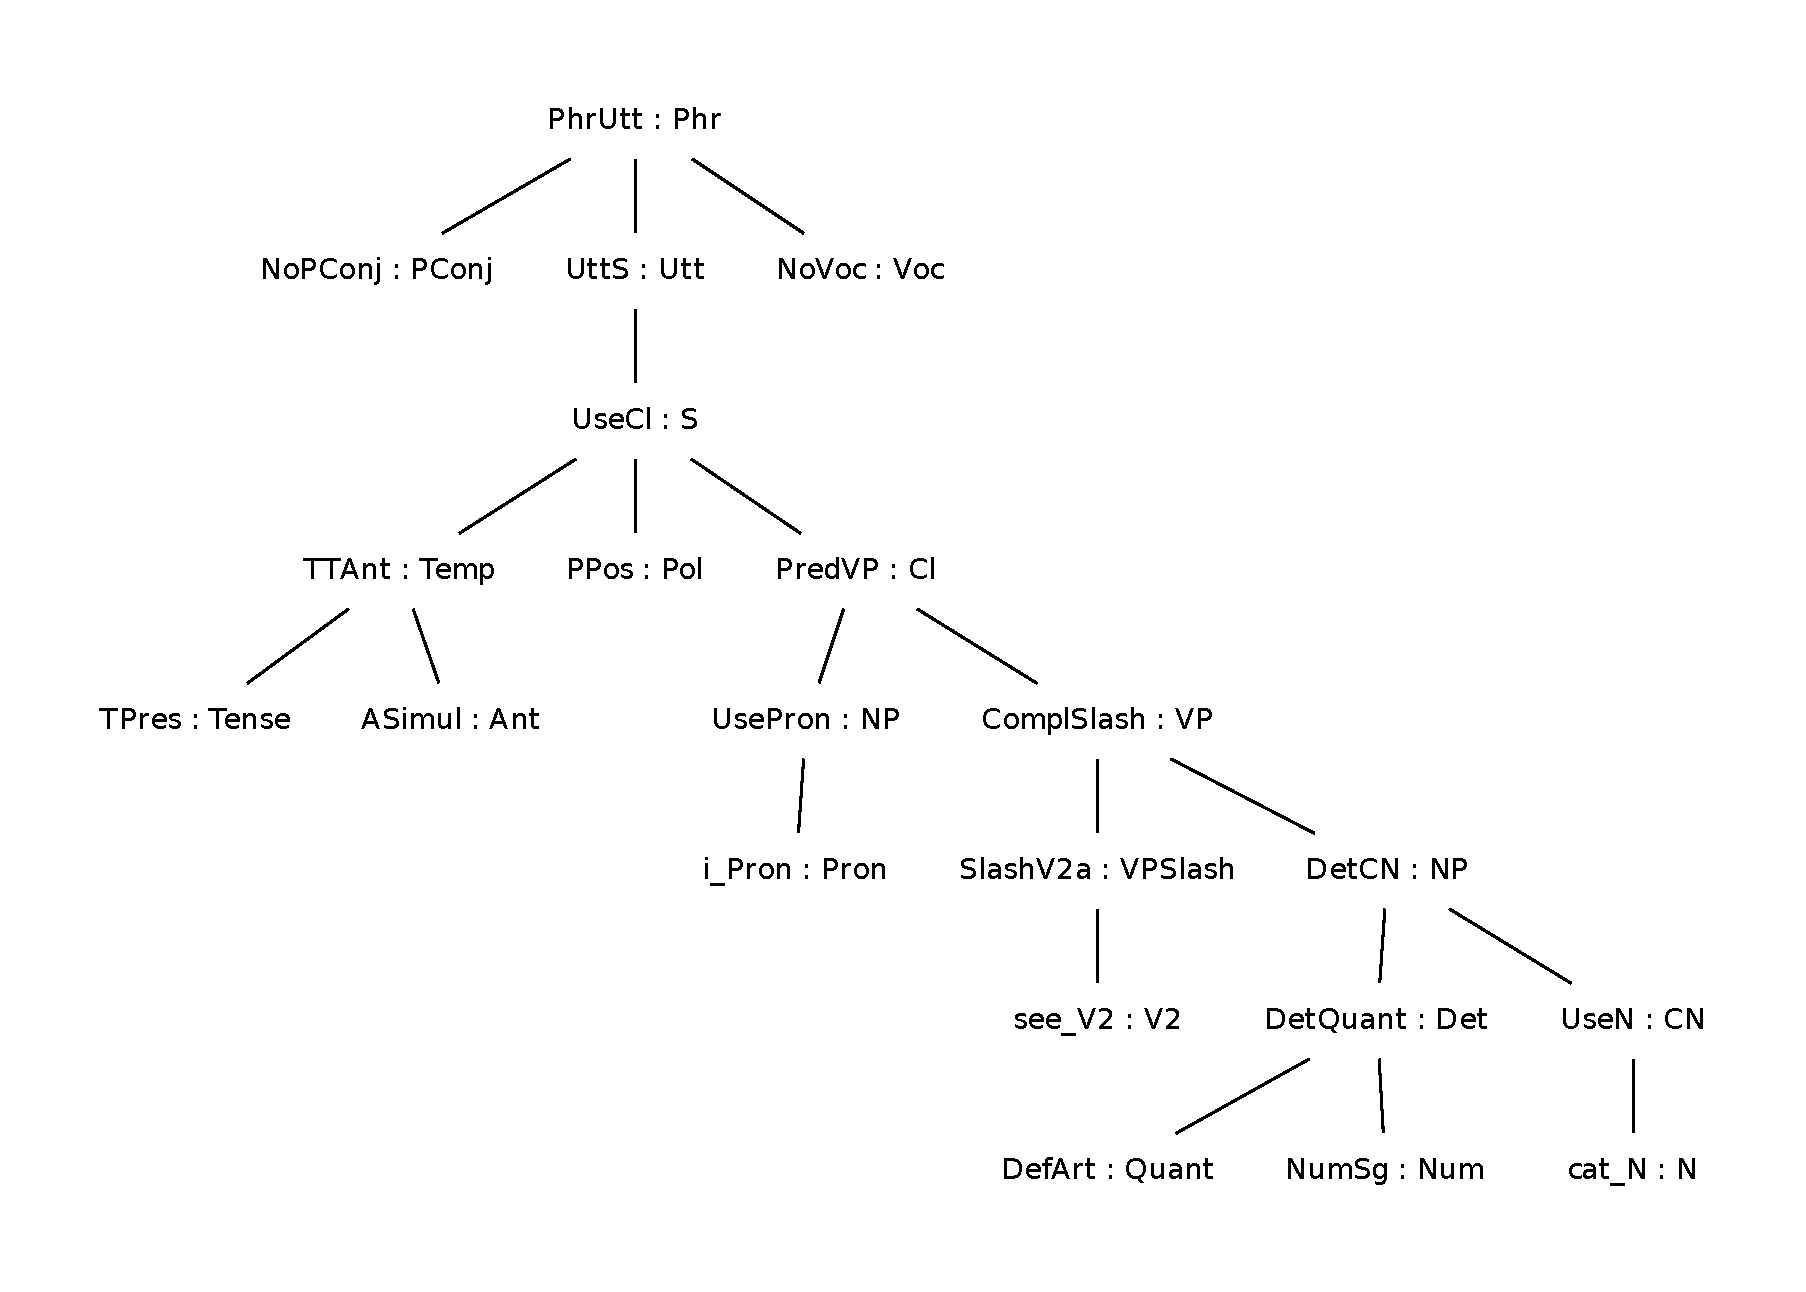
\includegraphics[width=100mm]{gfTree.pdf}}
\subfloat[Swedish parse tree]{\label{pic:gfStree}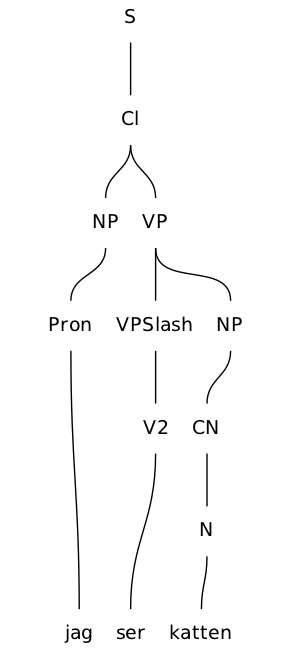
\includegraphics[width=30mm]{gfSTree.png}}
\caption{Abstract tree and parse tree for the sentence ``Jag ser katten".}
\label{fig:gftree1}
\end{figure}
\vspace{10mm}
% do not know about abstract/concrete yet: and is consequently the same for all concrete syntaxes.
The reader should keep in mind that the visualized parse trees is not a
complete representation. It does not reproduce all information from the abstract tree.
%If the end node of a  branch has no corresponding word, it is excluded from
%the visualized parse tree. This is the case for the 
For example, the definiteness and number of the noun \emph{`katten'}, which is shown as
\verb-DetQuant DefArt NumSg- in the abstract tree.
%and the information \verb-DetQuant DefArt NumSg- is not shown in figure \ref{pic:gfStree}.
In the corresponding English parse tree, figure \ref{pic:gfEtree},
the noun is explicitly quantified by the article \emph{``the"},
and the determiner is therefore shown in the parse tree.\\
%>> how parse trees work, not correct complete representation.
%>> not a constituent structure. compare to lfg, fstructure, cstructure.

%>>the scope is controlled language, but possible ambiguities (discuss this in future
%>>work, saldo, conclusion). Ambiguities: from multilinguality, or inherited:
%>>syntactical (man with the telescope), lexical (youSg/Pl, växa).
%>> have ambiguity section. 
\newpage
\begin{wrapfigure}{l}{0.35\textwidth}
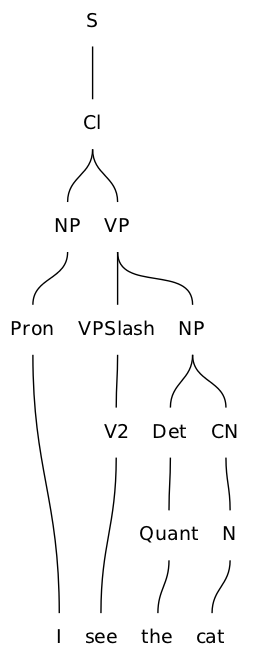
\includegraphics[width=30mm]{gfETree.png}
\caption{English parse tree}
\label{pic:gfEtree}
\end{wrapfigure}


%TODO read again
The scope of GF grammars has so far been controlled language, a limited
language used in a restricted domain. By
restricting the coverage, the number of ambiguities
can be limited and we can ensure that the semantics is preserved during
translation. Inherited ambiguities as well as ambiguities arising from multilinguality will
remain, but can be controlled more easily. %Example of domainspecific word?

The use of controlled language thus gives a possibility of good and reliable translation
and GF has successfully been used in project like %Some examples of projects using GF are 
WebAlt \cite{webalt}, a project which aims to develop language independent
material for mathematics problems. The formal software verification tool
KeY \cite{key}, in which GF is used for translating specification to natural language.
%>> key, talk, hats, bom (see references in Ramonas thesis).
%>> use talk here and move key to other place??
GF can be used for describe dialog grammars see \cite{talk}, and
the framework is further used in the
European project MOLTO \footnote{http://www.molto-project.eu/} for online
translation between up to 15 language.\\

\vspace{10mm}
\subsection{Writing a GF grammar}
\label{sec:writegf}
The key feature in GF is the distinction between
\textit{abstract} and \textit{concrete} syntax. The abstract syntax represents
the internal structure and models the semantics without concern for language
specific features such as agreement or word order.
An abstract grammar can be implemented by a set of concrete grammars, each
representing one language. As a comparison, the abstract and concrete syntax
may be thought of as f-structures and c-structures in Lexical Functional
Grammar \cite{lfg}.

%Being developed with multilinguality in mind, GF makes an important 
\begin{figure}[h]
\begin{verbatim}
 abstract TestGrammar = {
  cat N ; V ; S ;

  fun 
    Pred : N -> V -> S ;
    cat_N : N ;
    sleep_V : V ;
 }
\end{verbatim}
\caption{A small example of an abstract syntax}
\label{fig:gfAbstract1}
\end{figure}

The example in figure \ref{fig:gfAbstract1} shows an abstract grammar defining three categories, % \verb|Categories|,
one for nouns, one for verbs and one for sentences. The abstract grammar also gives
the function types. In this case we have \verb|Pred|, which tells us that by
taking a noun and a verb we can form a sentence.  No information of how this is
done is given at this stage. The grammar also defines two words, the noun
\verb|cat_N| and the verb \verb|sleep_V|. 

% or how any of the categories should look.
\begin{figure}[h]
\begin{verbatim}
concrete TestGrammarSwe of TestGrammar = {
  lincat N, V, S = Str ;
   
  lin Pred n v   = n ++ v ;
      cat_N   = "katten"  ;
      sleep_V = "sover"  ;
}
\end{verbatim}
\caption{A Swedish concrete grammar}
\label{fig:gfSweCnc1}
\end{figure}

%>> move much of this to Swedish GF part?
Figure \ref{fig:gfSweCnc1} shows how the abstract grammar can be implemented
for Swedish. Nouns, verbs and sentences are all defined as strings, \verb|Str|.
The function \verb|Pred| simply glues the two strings ``katten" and ``sover" together:\\
\verb|Pred cat sleep = "katten sover"|.\\
We get a more complicated example if we allow the nouns to be used in both
plural and singular. We add a category \verb|N'| to the
abstract, which represents a noun with a fixed number,
%Note that \verb-N'- is normally used for nouns with a fixed definitness, but for 
%now we concentrate on the number only. Hence \verb|N| now means a noun in any of the number,
and we introduce two functions that set the number: \verb|NSg : N -> N'| and
\verb|NPl : N -> N'|.
\begin{figure}[h!]
\begin{verbatim}              
 abstract TestGrammar = {          concrete TestGrammarSwe of TestGrammar = {
  cat N ; N' ; V ; S ;               lincat V, S, N' = Str ;
                                            N = {s : Num => Str} ;
  fun                                lin   
    Pred : N' -> V -> S ;              Pred n v = n ++ v ;
    NSg : N -> N' ;                    NPl n = n.s ! Pl ;
    NPl : N -> N' ;                    NSg n = n.s ! Sg ;
    cat_N : N ;                        cat_N = {s = table {Sg => "katten" ;
    sleep_V : V ;                                          Pl => "katterna"}};
 }                                     sleep_V = "sover"  ;
                                     param Num = Sg | Pl ;
                                     }
\end{verbatim}           
\caption{A modified grammar}
\label{fig:gfTest2}
\end{figure}
Figure \ref{fig:gfTest2} introduces some new concepts: records, tables and parameters.
In the concrete syntax, \verb|N| is defined to be a record consisting of the field
\verb|s|. The type of \verb|s|, \verb-Num => Str- shows that it is a table, which given a
parameter of type \verb|Num| returns a string. \verb|Num| is defined 
%as a parameter, which can
to either have value \verb|Sg| or \verb|Pl|. 
The dot (\verb-.-) is used for projection and the bang (\verb-!-) as a selection operator.
%In \verb|NPl| and \verb|NSg|,
\verb|n.s ! Sg| thus means that we use the branch for \verb-Sg- in
field \verb|s| of \verb|n|.
%, and then the selection operator \verb|!| is used to select a branch in the table.

When implementing an English version of the grammar, we encounter another
problem: the verb form depends on the number of the noun. We solve this by letting
\verb|N'| carry
information about its number and letting \verb|Pred| pass this on to the
verb. Finally, the type of \verb|V| is put into a table, showing the verbs forms for each
number.
\begin{figure}[h!]
\begin{verbatim}              
concrete TestGrammarEng of TestGrammar = {
  lincat S  = Str ;
         V  = {s : Num => Str} ;
         N  = {s : Num => Str} ;
         N' = {s : Str ; num : Num} ;
  lin   
    Pred n v = n.s ++ v.s ! n.num ;
    NPl n = {s = n.s ! Pl ; num = Pl} ;
    NSg n = {s = n.s ! Sg ; num = Sg} ;
    cat_N = {s = table {Sg => "the cat" ;
                        Pl => "the cats"}};
    sleep_V = {s = table {Sg => "sleeps" ; 
                          Pl => "sleep"}};
  param Num = Sg | Pl ;
  }
\end{verbatim}           
\caption{English implementation}
\label{fig:gfTestEng}
\end{figure}

%maybe continue example with swedish and english, have DetNP : N -> N wich
%gives 'the cat', 'katten'. Thereby introduce tables, parameters, fields.
%Show abstract tree.

We now have two implementations of the abstract, one for Swedish and one for English.
The resulting GF grammar is able both to
parse a string to an abstract tree and to go in the other direction; to produce
a string of natural language given an abstract tree. This step is called linearization.
Translation is a consequence of this, we can parse a Swedish string and then 
linearize the resulting abstract tree to English. 

\subsection{The resource library}
\label{sec:resources}
%>>Best part? Biggest library?
%>>Most general resource, first large grammar, covers fundamental syntactics.
The GF package provides an useful resource library \cite{gf-resource}, covering the
fundamental morphology and syntax of more than 20 languages.
There is also a small test lexicon included, containing a few hundred common
words.
%is a very useful part of the framework. It is provided in the 
%, they give a good start for all who want to write an application grammar.
%of a language for each application, all
%this can be found as libraries. So far there are 20 languages in the library, and
The languages all share the same abstract syntax which is  valuable
%they constitute  a very useful resource 
when implementing multilingual application grammars.

The resource grammars describe how to construct phrases and sentences and how to
decline words. The latter is done by smart paradigms: functions that analyse
some given forms of a word to find out how the inflection table should look.
For example, the declination of many Swedish nouns can be determined by looking
at the singular form only. 
\begin{wrapfigure}{l}{0.4\textwidth}
\begin{tabular}{| l | l |}
\hline
1st declination & 5th declination \\
\hline
flick\textbf{a}    &     hjärt\textbf{a}   \\
flick\textbf{an}    &    hjärt\textbf{at}  \\
flick\textbf{or}    &    hjärt\textbf{an}  \\
flick\textbf{orna}  &    hjärt\textbf{ana} \\
\hline
\end{tabular}
\end{wrapfigure}
This is the case for ``flicka", a noun belonging to the first declination. %the correct declination
%can be guessed by using the first declination. % and noting that the word ends with an ``a". 
%Like most Swedish nouns ending with an ``a", it follows the first declination.
For others, like "hjärta", also the plural form "hjärtan" is needed.
%, even though it ends with an ``a". 
The worst case is nouns that need four forms, both singular and
plural in definite and indefinite form.
Section \ref{sec:swegf} will give a more thorough description of the Swedish resource grammar.

\subsection{Frontiers of Grammatical Framework}
As an open source-project, GF is constantly being developed and improved. New
languages are added, the compiler is being improved, ways of using it in more 
efficient and easy-going manners are added
and the possibilities to use GF in different environments
increased. There is research on how to make more use of the dependent
types, for reasoning by using ontologies \cite{ontologies2} or generating natural
language via Montague semantics \cite{montague}.
%Further, experiments on using GF for free parsing has been conducted
%\cite[\textsection 4.1]{gfMech}.
%This is also a future goal for our project and one of the subgoal has been to
%model an important part of Swedish in GF. The starting point was the resource
%grammar to which the result has a strong connection.

%Functor
%Main ideas, abstract and concrete, translation, parse- and abstract trees.
%We say that this is a function that takes as argument and returns..
%Categories, valency built in (problems with ställa - på, under, vid). Parameters, fields.
%Example of a piece with Swedish, the reader gets familiar with how it looks.
%Also show how information 'disappears', become strings.
%What kind of linguistic analyse, what is the purpose to cover. Mention other uses,
%ideas of anaphores, montague? dependent types, ontologies, cool pictures by Krasse.
%
%The resources, why, how many, how to use, projects. functors.
%
%Still under big development, evolving, growing.
%For this project, only (mostly) important to model Swedish without abandoning the
%resources too much. Use of the big grammar for translation, why it might be hard with
%semantics and lexicon.
%Research about how to parse with gf by Krasimir, experiments with English.

%inte vet jag. foc + v + resten

\section{Talbanken}
\label{sec:talbanken}
For testing and evaluation of the grammar and lexicon, we needed to be able to
compare them against a reliable source.
Talbanken \cite{talbanken} was perfect for our purpose,
being a freely available, manually annotated, large-scale treebank.
%It was created in the 1970s at Lund University.
It is analyzed with the MAMBA annotation scheme (Teleman, 1974) and 
consists of four
parts. Two of them are transcriptions of spoken language, one a collection of
text written by high school students, and one, section P,
consists of professionally written Swedish gathered from newspapers, brochures and textbooks.
\\
Talbanken was also used to train the Swedish version of the Malt parser \cite{malt}
and was then redistributed in an updated version,
Talbanken05 \cite{talbanken05}.
%This work was done by Nivre, Hall and Nilsson in 2005.
It is released in Malt\footnote{http://w3.msi.vxu.se/~nivre/research/MaltXML.html} 
and Tiger\footnote{http://www.ims.uni-stuttgart.de/projekte/TIGER/TIGERSearch/doc/html/TigerXML.html}
XML-formats
where the trees had been made deeper and more detailed while still containing
the lexical MAMBA layer. \\
The Malt parser was trained on section P of Talbanken, and these
more than 6000 sentences have been used our project. 
The treebank has served as an inspiration and an evaluation source throughout the
project. An automatic mapping between its trees and the abstract trees from GF has been
done, which will be explained in section \ref{sec:Mapping}.
%Differences in analyse, do we want a similar? 
%Uses of Talbanken in project, mapping to evaluate and test.  
%Look at output from Maltparser, could also comparing our parse trees to this.


\section{Saldo}
\label{sec:saldo}
A good parser needs a good lexicon. We have used Saldo \cite{saldo}, a
large electronic lexicon developed and maintained at Gothenburg University. It is
built on Svenskt Associationslexikon and contains information about more than 
120 000 modern Swedish words.
For each word there is semantic, syntactical and a morphological
information. The user can find examples of usage in corpora,
graphs of semantically connected words and some suggestions for how to analyse compounds. \\
\begin{figure}[h!]
\centering
\subfloat[Morphological info for ``katt"]{\label{pic:saldoTab}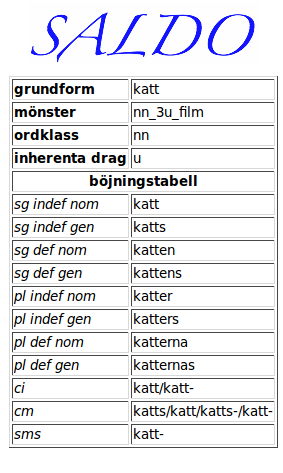
\includegraphics[width=40mm]{saldotab.png}}
\hspace{20mm}
\subfloat[Graph showing the hyponyms of ``katt"]{\label{pic:saldoWheel}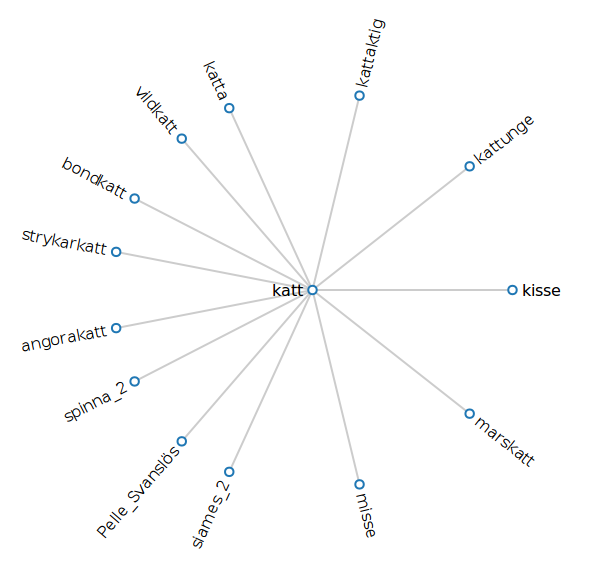
\includegraphics[width=70mm]{saldograph.png}}
\caption{Information in Saldo}
\label{fig:saldo}
\end{figure}

The semantic aspect of Saldo requires that words with multiple meanings are
separated into different entries.
%TODO change word? uppskatta, känna, få
The word ``växa" (``grow") for example, has two meanings: \emph{getting
bigger}
\enumsentence{Gräset växte varje dag\\
`The grass grew each day'}
or \emph{being a plant}. 
\enumsentence{Det växte en gammal ek där.\\
`There stood an old oak.'}
``växa" is however declined the same way for both interpretations of the word.
Hence \textit{Saldo's morphological lexicon} only keeps one entry of ``växa".
For the homonyms that do not share the whole inflection tables, different entries are 
kept also in the morphological lexicon.

For our purpose, only the morphological section, provided under LPGL in XML
format, was needed.
The data can be processed and translated to GF format as described in 
section \ref{sec:prog.saldo}.

\section{Swedish}
\label{sec:swedish}
Swedish \cite[Inl. \textsection 3]{SAG}is a North-Germanic language,
closely related to Norwegian and Danish. The languages share most of their
grammatical structures and are mutually intelligible. Swedish is also 
one of the official languages in Finland and altogether spoken by approximately 9
million people.
Swedish syntax is often similar to English, but the  morphology is richer and the
word order slightly more intricate.

\subsection*{Post-nominal articles} 
\label{sec:swedishnoun}
Unlike most of the world's languages Swedish express not only the number but also
the definiteness of a noun by suffixes. The endings are decided by the noun's gender,
%which may be 
\textit{neuter} or \textit{non-neuter}.\\
%(or \textit{utrum}) 
\begin{tabular}{l|lll}
                  &\textbf{Indefinite} & \textbf{Definite}& \textbf{Gender} \\
 \hline
\textbf{Singular} & {en katt}        & {katten}           & \textit{non-neuter}\\
                  & \emph{a cat}     & \emph{the cat}     &\\
\textbf{Plural}   & katter           & katterna           &\\
                  &\emph{cats}       & \emph{the cats}    &\\
 \hline
\textbf{Singular} & {ett hus}        & {huset}            & \textit{neuter}\\
                  & \emph{a house}   & \emph{the house}   & \\
\textbf{Plural}   & hus              & husen              & \\
                  & \emph{houses}    & \emph{the houses}  & \\
\end{tabular}\\

%The definiteness can be accentuated by using the definite articles.\\
%\begin{tabular}{llll}
%den katten & det huset & de katterna & de husen \\
%\emph{the cat} & \emph{the house} & \emph{the cats} & \emph{the houses} \\
%\end{tabular}\\

A definite article or a determiner is necessary when the noun is modified by adjectival
phrase; sentence (\ref{sent:trottkatt}a) is not grammatically correct.
As adjectives also marks definiteness, this is marked on three places
in sentence (\ref{sent:trottkatt}b). %, the definiteness is 
%The definiteness in then marked by the article, on the noun and on the adjective.

\enumsentence{\begin{tabular}[t]{@{}*{10}{l@{\ }}}   %\begin{tabular}[t]{@{}*{lllllll}}
a. & *Gamla          & katten        &sov. &&b. &Den             &gamla            & katten         &sov.\\
   & $[${\sc+def}$]$ & $[${\sc+def}$]$&    &&  & $[${\sc+def}$]$ & $[${\sc+def}$]$ & $[${\sc+def}$]$&  \\
   &~~`The old       & cat           &slept.'&& &`The            & old             & cat            &slept.'\\
\end{tabular}}\label{sent:trottkatt}
However, for some determiners, ie. `min' (\emph{`my'}), the noun should be in indefinite form.
%the definitness of the noun is set by the determiner. For some,
%like `min' , the noun should be used in indefinite form.

\enumsentence{\longexnt{3}{3}
{min &trötta& katt} %&& Den där & trötta &katten}
{`my & tired & cat'}
{ $[${\sc+def}$]$ &$[${\sc+def}$]$& $[${\sc-def}$]$} % . && $[${\sc+def}$]$  & $[${\sc+def}$]$ &$[${\sc+def}$]$}
{}}

%a.& Katten& sov. & b
% &$[${\sc+def}$]$ & %can be superdoubled
%  &`The cat& slept.'%example: den där boken


\subsection*{Verb second}
Swedish is a verb-second language \cite[p.116]{gunlog}: the
second constituent of a declarative main clause must consist of a verb.
The normal word order is subject-verb-object, but any syntactic category can be
fronted \cite[\textsection 1027]{H&H}.
This is called topicalisation and is very common, especially for temporal and
locative adverbial phrases.
The examples \ref{ex:swedish-svo} - \ref{ex:swedish-avso} all have the same propositional
meaning, but vary in how the content is presented.
%~~ although the fronted part of sentence (\ref{ex:swedish-ovs}) and (\ref{ex:swedish-avso}) are being
%emphasized.
\enumsentence{
\shortex{4}
{Du & ser &  inte &mig.}
{\emph{you} & \emph{see} & \emph{not} &\emph{ me}}
{`You  don't see me'.}} \label{ex:swedish-svo}
\vspace{-3mm}
\enumsentence{
\shortexnt{4}
{Mig  & ser &  du & inte.}
{\emph{me} & \emph{see} & \emph{you} &\emph{ not}}}\label{ex:swedish-ovs} 
\vspace{-3mm}
\enumsentence{
\shortexnt{4}
{Inte & ser& du &mig.}
{\emph{not}&  \emph{see}& \emph{you}& \emph{me}}} \label{ex:swedish-avso}

%Alla syntaktiska kategorier kan be fronted utom obetonade satsadverbial (ju,väl).
%\enumsentence{
%\begin{tabular}{lll}
%  Johan & gick & sakta på gatan.\\
%\emph{Johan} & \emph{walked} & \emph{slowely on the street.}\\
%  Sakta & gick & Johan på gatan.\\
%\emph{Slowly} & \emph{walked} & \emph{Johan on the street.}\\
%  På gatan & gick & Johan sakta.\\
%\emph{On the street} & \emph{walked}  & \emph{Johan slowly.}\\
%\end{tabular}}

Inverted word order marks questions
\enumsentence{
\shortex{4}
{Såg & du & mig & inte?}
{\emph{saw}  & \emph{you}&  \emph{me}& \emph{not}}
{`Didn't you see me?'}}
%\enumsentence{Gick Johan på gatan?\\
%        \emph{Did Johan walk on the street?}}
The word order in subordinate clauses in also slightly modified,
%>> and stricter
\enumsentence{Main sentences:\\
{\shortex{8}{Jag & såg & Anna & men & hon & såg & {\bf inte} & mig }
{ \emph{I} & \emph{saw} & \emph{Anna} & \emph{but} & \emph{she} & \emph{saw} & {\bf \emph{not}} &\emph{ me}}
{`I saw Anna but she didn't see me'}}}
\enumsentence{Subordinate sentence:\\
\shortex{7}{Jag & förstod & att& Anna& \textbf{inte}& såg& mig.}
            {\emph{I} &  \emph{understood} & \emph{that}& \emph{Anna}& \textbf{\emph{not}}& \emph{saw}& \emph{me}}
            {`I understood that Anna didn't see me'}} 

\subsection*{Passive voice}
There are two ways of forming passive verb phrases in Swedish: the 
\textbf{periphrastic passive}, formed by using the modal auxiliary verb `bli' (\emph{`become'}).\\
%>> better with animate subjects
\enumsentence{
\shortex{5}
{Tjuven &blev& tagen& av & polisen}
{\emph{the} \emph{thief} & \emph{was} & \emph{taken} & \emph{by} & \emph{the police} }
{`The thief was arrested by the police'}}
\label{gfPass:peri-pass}
and the \textbf{s-passive} which is formed by adding an \emph{s} to the verb: \\
\enumsentence{Passive \hspace{45mm} Active\\
\shortexm{12}
{Tjuven & togs&  av & polisen}
{\emph{the}\emph{ thief}&  \emph{took}+\textbf{s}&  \emph{by}&\emph{the police}}
{`The thief was arrested by the police'}
{&&Polisen & tog & tjuven}
{&&\emph{the police} & \emph{took} & \emph{the thief}}
{\hspace{-9mm}`The police arrested the thief'}}
\label{gfPass:s-pass}
The s-passive is more commonly used than periphrastic passive, for both written
and Swedish \cite[Pass. \textsection 1]{SAG} and dominates especially when the subject is inanimate.
%cf.
%\enumsentence{
%\shortex{5}{Ett & lejon & jagade & honom.}
%        {A &lion &hunted &him.}
%        {`A lion was hunting him.'}}

\subsection*{Impersonal constructions}
Constructions with `det är/var' (\emph{`it is/was'}) \\are very common in Swedish
\cite[\textsection 309d]{H&H}:
\enumsentence{
\shortex{6}{Det & var & roligt & att & höra.}
{\emph{it} &\emph{was} & \emph{nice} &\emph{to} &\emph{hear}.}
{`I'm glad to hear that.'}}
'Det' %(\emph{it})
is also used as formal subject in presentational constructions where
the real subject is put in the position of an object.
\enumsentence{
\shortex{6}{Det &står &en &älg &på &fältet.}
{ \emph{it} & \emph{stands} &\emph{a} & \emph{moose} &\emph{on} &\emph{the field}}
{`There is a moose in the field.'}}

\subsection*{Reflexive pronouns}
\label{swe:refl}
The Scandinavian language have special reflexive pronouns
and reflexive possessive pronouns for the 3rd
person \cite[\textsection 310 \& 319]{H&H}, distinct from the normal 3rd person forms.
\enumsentence{
\begin{tabular}{llll}
a. & Han slog \textbf{sig}.&\hspace{20mm}b. & Han såg \textbf{sitt} barn.\\
&\emph{He hit him self.} && \emph{He saw his (own) child.}
\end{tabular}}
\enumsentence{
\begin{tabular}{llll}
a. &Han slog \textbf{honom}. &b.& Han såg \textbf{hans} barn.\\
&\emph{He hit him (another person).}&&\emph{He saw his (another person's) child.}
\end{tabular}}
The 1st and 2nd persons use the normal personal pronoun in object form as reflexive
pronouns.

%Mention varandra. Same idea.
%Basic info about Swedish. V2 lang, inverted word order and subordinate clauses.
%Passive, reflexive 'sitt', 'det är', 'det sitter en katt där', prepare the reader
%for what will be written in the grammar part.
%Adjectives but not verbs congruate with nouns. De är stora, They are big, Jag
%är stor, I am big
%Since the s-passive is the most common one in written Swedish \cite{SAG-34-1}, it has


\section{Related work}
\label{sec:related}
%There has been much research about parsing Swedish. INTRO!!
Many years of research have lead to many interesting language
technology tools for Swedish.
An example is the well-known data-driven Malt parser \cite{malt},
which has been trained on Talbanken. 
There are also a number of grammar-based parsers, although none is freely available.
The cascaded finite state parser CassSwe \cite{casswe} and
The Swedish Constraint Grammar (Birn,1998) 
give syntactic analyses. %birn: shallow
Swedish FDG (Voultanien,2001) uses the Functional Dependency Grammar
(Tapanainen and Järvinen,1997), an extension of the Constraint Grammar
formalism, and produces a dependency structure focusing on finding the nominal
arguments. \\
%for the  finding subject, objects, suubject complements (SC) and
%to link them to their proper regents (main verbs) : over 90 \% both precision and recall.

%Tag, Tree adjoining grammar, XTAG: English and Korean, Chinese? English:
%ongoing to get widecoverage grammar
%under GPL. Translation to Korean.

The LinGO Grammar Matrix \cite{matrix}, is a starter-kit for building Head-Driven Phrase
Structure Grammars \cite{hpsg} (HPSG) providing compatibility with tools for
parsing, evaluation, semantic representations etc.
Translation is supported by using Minimal Recursion
Semantics \cite{mrs} as an interlingua. \\
There is a collection of grammars implemented in this framework, giving broad-coverage
descriptions of %broad-coverage
English, Japanese and German. %, Greece, Spanish etc. 
The Scandinavian Grammar Matrix \cite{scandmatrix} covers common parts of
Scandinavian, while Norsource (Hellan, 2003) describes Norwegian. A Swedish version
was based upon this (SweCore, Ahrenberg) covering the morphology and some
differences between Swedish and Norwegian. Further, there is the BiTSE 
grammar \cite{stymne}, also implemented using the Lingo Matrix,
which focuses on describing and translating verb frames.\\ % and translating them to English. \\

%It should be pointed out that grammars implemented using Lingo Matrix
%do not share any common abstract, like the resources grammars of GF?\\

The Swedish version of the Core Language Engine (CLE) \cite{gamback} % \cite{cle}
gives a full syntactic analysis as well as semantics represented in `Quasi logical form'. A
translation to English  was implemented and the work was further developed in the spoken
language translator \cite{spoken}. Unfortunately, it is no longer available. The coverage of the Swedish
CLE is also reported to be very limited \cite[p. 134]{nivretrees}.\\

In the TAG formalism \cite{tag}, there are projects on getting open source, wide-coverage grammars
for English and Korean, but, to our knowledge, not for Swedish.  \\

The ParGram \cite{pargram} project aims at making wide coverage grammars using
the Lexical Functional Grammar approach \cite{lfg}.
The grammars are implemented in parallel in order to coordinate the analyses of
different languages and there are now grammars for English, German, Japanese and Norwegian. 


%However has been two, about CLE \cite{cle} and what happened to it. Logic and translation
%to Swedish, S-CLE (Gambäck,1997) full analyse and semantics, translation,
%but coverage is too limited (nivres papper), The
%spoken lang. translator \cite{cle2}. 

%>> Much more here, important!! comparisons.
%>> HPSG and LFG are context sensitive
%Computational ling is active area for Swedish, there are many other Swedish parser,
%but grammars?
%Many of the parsers not ruled based, the most known one Malt \cite{malt} ... .
%Wiren \cite{wiren}?? chartparser, but for
%swedish. bit more information than just pos: cassSwe \cite{casswe}
%Other Sw. parsers and grammars, evaluation of them? 
%Other grammar frameworks.
%SweCG (birn) annotation, parser Swedish FDG  (voultanien,2001)which is not
%freely available.
%finding subject, objects, subject complements (SC) and
%to link them to their proper regents (main verbs) : over 90 \% both precision and recall.
%uses a dependency grammar, but "The functional description of adverb phrases
%and prepositional phrases (e.g. agent, source, goal, benefactive, time) remains
%to be described in a future version." 
%HPSG \cite{hpsg} and lingo matrix , English, Japanese, German,
%Greece, Spanish, Norweigan (NorSource, Hellan 2003),( not famous: SweCore
%(Ahrenberg) based on NorSource)
%also Swedish: BiTSE \cite{stymne}, Stymne 2006, Swedish English translation,
%and one for the common parts of scandinavian (Haugereid etc) in Nordisk sprog.
%focusing on verb phrames, built on HPSG.
%S\o rgaard and Haugereid, Scandinavian Grammar Matrix \cite{scandmatrix}
% related and references work: CLE, Krasimirs book, CassSwe, GF book,SAG, gunlög,
% the multilingual treebank, Homse&Hinchcliff, Aarne i LILT

\chapter{Importing Saldo}
\label{sec:prog.saldo}
The lexicon provided with the GF resources is far too small for open-domain parsing.
Experiments have been made to use an interactive tool for lexical acquisition,
%but the dictionary was still much to small. The acquisition tool may still
but this should be used for complementing rather than creating the lexicon.
This section describes the process of importing Saldo, which is 
compatible with GF, and easily translated to GF format.
As Saldo is continuously updated, the importing process has been designed to be fast
and stable enough to be redone at any time.

\section{Implementation}
%>> syntactic information too. Mention that GF does not have this, only lexical or
%>> semantic. Not 1-1.
The basic algorithm for importing Saldo was implemented by Angelov (2008)
and  produces code for a GF lexicon.
For each word in Saldo, it decides which forms should be used as input
to the the GF smart paradigms. For a verb, this will in most cases mean giving
the present tense form, see figure \ref{fig:saldoknyt}. \\

\begin{figure}[h]
\verb-mkV "knyter" ;-
\caption{First code produced for the verb `knyta' (\emph{`tie'})}
\label{fig:saldoknyt}
\end{figure}

All assumed paradigms are printed to a temporary lexicon, 
which will produce an inflection table for every entry when compiled.
The tables are compared to the information given
in Saldo, if the tables are equal the code for the word is saved. If the table
is erroneous, another try is made
by giving more forms to the smart paradigm.
For example \ref{fig:saldoknyt}, the smart paradigm will fail to calculate the
correct inflection table. In the next try both the present and the past tense
are given:\\

\begin{figure}[h]
\verb-mkV "knyter" "knöt" ;-
\caption{Second output for the verb `knyta'}
\label{fig:saldoknyt2}
\end{figure}
The program is run iteratively until the GF table matches the one given in Saldo,
or until there are no more ways of using the smart paradigm. The verb 'knyta'
will need tree forms:\\

\begin{figure}[h]
\verb-mkV "knyter" "knöt" "knutit"-\\
\caption{Final output for the verb `knyta'}
\label{fig:saldoknyt3}
\end{figure}

%Find the paper!
%The program will try to create a lexicon by finding a number of forms for every
%word and feeding them to the smart paradigms. As few forms as possible should be
%used, and the resulting table generated by GF should be equivalent to the one found
%in Saldo. This process is done iteratively,
%starting from the easiest case. For each attempt the results are compared and when
%the correct way of using a word has been found, the code is saved.

Figure \ref{pic:TabVax} shows the information given by Saldo and by GF respectively.\\
\begin{figure}[h]
  \begin{center}
\subfloat[Saldo]{\label{pic:saldoVax}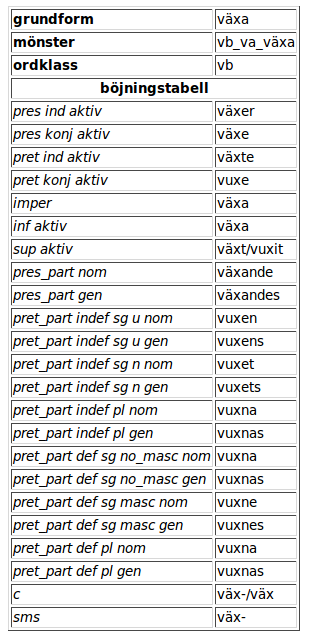
\includegraphics[height=90mm]{saldoVax.png}}
\hspace{5mm}
\subfloat[GF]{\label{pic:gfVax}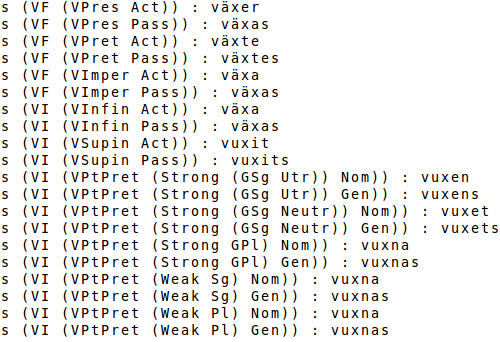
\includegraphics[height=60mm]{gfVax.png}}
\caption{Inflection table for the verb ``växa" (grow)}
\label{pic:TabVax}
  \end{center}
\end{figure}
The tables does not overlap completely, there are some more forms in Saldo's table (e.g. the 
compounding form ``väx-")
while the one generated in GF contains some that are not in Saldo (e.g. ``vuxits").
As GF concerns about syntax only, and not semantics, and  as the GF tables are automatically
generated, they always contain all word forms, although some forms may never be
used in the natural language.
Saldo may also contain variants: ``växt" and ``vuxit" are both supine form.
As far as possible, the program makes up for this by only comparing the overlapping forms
and only requiring that GF generates one variant whenever alternatives are given. \\
%The program continues to generate new lexicons as long as there are more
%paradigms to choose from and compare the results after each run.

During this project, the program has been made more robust than the previous
version. It also prints log files providing
information about the process of importing each word: which paradigms that have been
tried, the results from the comparisons of the inflection tables and finally listings
of the words that could not be imported.

Each entry in Saldo has an identifier, e.g. \verb-äta..vb-, which is used as 
constant names in the GF lexicon. However, the identifier may need some renaming since
the there are special characters  in the Saldo identifiers
that should be avoided in GF function names. The importation therefore
needed some renaming. The Swedish letters \emph{å,ä,ö} are translated into
\emph{aa,ae,oe} respectively. 
\begin{verbatim}äta..vb  -> aeta_V \end{verbatim}
This translation may cause two or more lemmas to share the same
GF identifier, and to avoid name collision a number is added to the name
whenever a translation have been done: 
\begin{tabular}{lll}
kältisk & $\rightarrow$ & kaeltisk\_1 \\
kaeltisk & $\rightarrow$ & kaeltisk \\
entrecôte &$\rightarrow$ & entrecoote\_1 \\ 
\end{tabular}\\

%Problems with naming convention, special
%characters (å,ä,ö,apostrop,entrecôte.) needs to be translated , but avoid
%classhes 'kaeltisk' 'kältisk', gf will crash by this, so we add a 1
%in the end whenever we have changed a letter.
%,é
%Costs very much memory, the saldo file is big, the generated lexicon is big.
%Saldo is divided to save memory. Errors should just be reported, but if something oförutsett
%happens and one part fail, the separation ensures that the others wont, also
%possible to restart. 

%Explanation of the algorithm: map categories, try each paradigm, compare the table of forms
%created. If several forms in saldo, gf should pick on of them. Saldo has forms for
%compounds, gf does not. A grammar is written, the correct ones saved, the others 
%retried. Try all paradigms which can be formed from saldo. 
%In Saldo there is also semantic info, so
%We need the numbers from saldo if there are to lemmas with the same
%identifier. växa (bli större), växa (vara en planta) vs. sluta\_V and sluta2\_V
%(slöt). However gf does not want more than one table
%if the forms are identical, saldo's morpho neither, but there are five in big saldo. 
%We are just interested in morphology, so far. Dont want too big lexicon.

%see notes to add more about this, pronouns and the importing itself
%choices for adjectives vs. verbs for particips


\section{Results}
\label{sec:saldoRes}
The resulting dictionary contains more than 100 000 entries, approximately 80 \% 
of the total size of Saldo.
There are a number of reasons why some words were not imported,
the most obvious one is that we do not want all categories from
Saldo in the GF lexicon. Prepositions, %(\emph{pp})
numerals %(\emph{nl}),
personal pronouns etc.
are assumed to be present in the resource grammars and should not be added again.
Saldo contains many pronouns which
are not analysed the same way in GF (see section \ref{sec:swegf}).
Befor adding them to our lexicon, we need to do more analysing to find their correct GF-category.
%TODO read again
%They can thus not simply be extracted -- we first need to find their correct GF category.
Some experiments on finding the category
%the right GF-category for those
have been done using Talbanken, see p. \pageref{sec:gf.quant}.

%and are usually not kept in the standard lexicon, but in modules for the basic
%structures of the language.
Categories involving multiple words %(\emph{vbm, nnm})
are usually handled as idioms and should be given in a separate lexicon. In
total six categories were imported: \\

\begin{figure}[h]
\begin{tabular}{|l|lll|}
\hline
& Saldo tag & GF category & Example \\
\hline
 Adverb & \textbf{ab} &\textbf{Adv} & ofta (\emph{often})\\
 Adjective&\textbf{av} &    \textbf{A} & gul (\emph{yellow})\\
 Noun & \textbf{nn} &\textbf{N} & hus (\emph{house})\\
 Verb & \textbf{vb} &\textbf{V} & springa (\emph{run})\\
 Reflexive verbs  &\textbf{vbm}& \textbf{V} & raka sig (\emph{shave})\\
 Verbs with particles &\textbf{vbm}& \textbf{V}  &  piggna till (\emph{perk up})\\
\hline
\end{tabular}
\caption{}
\end{figure}

%
%There are a number of differences between and saldo Till skillnad från GF,
%saldo does not contain forms that aren't used gf generates all forms. A form
%needed to generate the gf table may not be given in saldo such as singular
%forms for 'byxor'. Also contains idioms, 'hålla huvudet kallt' and has
%different grammatical analyse, a lot of pronouns. Example. 
Most but not all words of the categories listed above have been imported.
One reason why the importing phase would fail 
is that Saldo, unlike GF, only contains the actually used word forms.
% does not contain information about ~~word forms that are not used~~.
For technical reasons, the smart paradigm might need forms never used.
%for this is Deponent verbs
%are for example given with their (often non-existing) active form, al
%In some cases those forms are needed by the smart paradigm. 
Consider for example
the plural tantum % \cite[44]{SAG} 
noun \emph{``glasögon"} (\emph{``glasses"}).
The smart paradigm requires a singular form, and since the program could not
find this in Saldo, there was no way of adding the lemma to the lexicon. 
When the program failed to import a noun, this was often the explanation.
%bbMany nouns fai, \emph{``kläder"} (\emph{``clothes"} etc.
Words of this type may be added manually, for \emph{``glasögon"} we could use
the ostensibly correct singular form ``glasöga", although this
has another meaning (``glass-eye").
The same problem occurred for the irregular s-verbs,
(\emph{``synas"} \emph{(``show")} or \emph{umgås} \emph{(``socialize")})
which made up 61.5 \% of the failing verbs of type \verb_vb_.\\
%``frodas" (``flourish"), ``lyckas" (``succeeed").
In a few cases the smart paradigms could not generate the correct declination.\\

%although this happened seldom. The passive preteritum is an exapmle of a form 
%oftenly because the one form could not be generated. anbd for passive preteritum could not be guessed.
%that seems hard to guess for some verb.
% >> should we add smth for this?
%\begin{tabular}{3}
%&\textbf{Saldo}& \textbf{GF}
%\textbf{Passive preteritum} & fryses & frys \\
%\end{tabular}
%>> exapmles: % frysa,fisa passive preterium 

%compared to the total size of Saldo this is .
When testing the coverage of Talbanken,
we found that there are around 2500 word forms still missing, excluding the ones
tagged as names and numbers. This number may seem very high, but %considering that
4/5 of the word forms are compounds and when performing the intended parsing,
these an additional analysis before being looked-up in the lexicon. We
should also take into consideration that 
we cannot automatically find out how many actually stem from the same word, or
how many abbreviations that are present (Talbanken also contains a small number of 
spelling errors, which probably are enumerated among our missing words). The majority
of the missing words are only used once.\\

\begin{figure}[h]
\begin{tabular}{|l|l|}
\hline
Missing words & $\sim$ 2500 word-forms\\
Missing words, ignoring compounds & $\sim$ 500 word-forms\\
Missing words used more than once & $\sim$ 500 word forms\\
Missing words used more than once, ignoring compounds & $\sim$ 150 word-forms\\
\hline
\end{tabular}
\caption{}
\end{figure}

%       The table suggests that many 
%       >> 2537 without IDs and only the ones built of Alpha,only 552 without compounds, still contains abbrev.
%       >> 494 without abbr. spelling errors
%       >> 142 more then one time.
%       numerals and proper names, but some names are still there). In addition, there were 1817 words
%       >> 223 were IDS.++146 HS.
%       >> 426 more than one time, with compounds.
%       >> give reasons! should look good, not bad!
A list of words that were given different labels in GF than in Talbanken has been
composed, consisting of about 1600 entries. Many of those are
acceptable and reflects the difference 
made in the analyses, such as the examples in table \ref{tab:saldodiff}.
Others are examples of words that are still missing from
the lexicon.
\begin{figure}[h]
\begin{tabular}{|lll|}
\hline
Word    & Talbanken tag & GF category \\
\hline
måste   & MVPS          & VV \\
allting & POTP          & N \\
få      & POZP          & Det \\
\hline
\end{tabular}
\caption{}
\label{tab:saldodiff}
\end{figure}

%Since Saldo does not give any valency information, neither does the imported lexicon.
%The lexicon does not contain any information.
Valency information, which is crucial for GF, is not given in Saldo and
hence not in the imported lexicon. It remains as future work to find methods 
%using the results from the mapping (see section \ref{sec:Mapping})
to extract this information from Talbanken and to automatically build
it into the lexicon. 
%The saddest thing: no valency info. Crucial for GF. Only reflexive and verbs with particles
%have any information. The earlier explained techniques may be used for this in Talbanken.
%To get even bigger material, use Korp, but then no guarantee.


\chapter{The grammar}
\label{sec:prog.grammar}
An important part of this project has been to develop the Swedish GF grammar and
to adapt it to cover
constructions used in Talbanken. As a grammar implementation can never be
expected to give
full coverage of a language, we aim for a grammar fragment which gives a deep
analysis of the most important Swedish constructions.
The starting point has been the GF resource grammar and the new implementation is
still compatible with this.
Before describing the actual implementation in section \ref{sec:Added}, we will give an introduction to the
resource grammars in general and to the Swedish implementation in particular.
%This is found in section \ref{sec:swegf} while section \ref{sec:Added} shows and
%explains the development during this project.

%We can't expect to get a grammar giving full coverage, instead we aim for a
%grammar that gives
%a deep analysis while having a satisfactory coverage.
%The starting point has been the Swedish
%resource grammar and the new grammar should still be compatible with this.
%%A description of the Swedish implementation of the resource grammar is given
%%in the next section, while
%Before describing what has been added, will give a short introductions to the
%the cats of resource grammar and the sw implementation in particular.
%This is done in section%Explain what's in the resources, constructions present in most languages. 
%Been working on a grammar fragment based on Talbanken,
%like cool people like Montague. May also be interesting for other purposes.
%Swedish shares with Nor and Dan. Extra module, covering things like sw is a
%v2-lang, focusing parts of sentences. 


\section{The Swedish resource grammar}
\label{sec:swegf}
%>> start by easy examples, jag ser inte dig, du ser inte mig osv. 
%>> plocka från svenska delen 1 2 4 
%>> show simple trees
%>> explain all in Sw. section.
%>> show abstract and concrete tree, compare. (or in Gf sect)
%>> no subjects or object, analyse is more from the lexicon,
%>> compare to others, ask elisabet.\\
%>> gf has pos-driven, leads to part-of-sentence analyse. first have v2,a2,vs etc.
%>> they may be combined in traditional way, and so the types depend and relate to each other
%>> see slides from summer school.
%>> worked well until now, but particular langs. needs particular solutions. --> reflexives!
%>> no syntactic theory can cover a whole language, and so gf can't either.


% TODO!
%>> functions for predication, complementation.
%>> rather different from others syntactical theories. does not remember syntactical
%>> parts of sentences, like subj, obj, attributes.
%>> shares 80 \% with scandinavian, mostly words that differ.\\
%>> complete morphology, limited syntax\\

The GF resource grammars gives a fundamental description of Swedish,
covering the morphology,
word order, agreement, tense, basic conjunction etc.
 %and many phrase and clause constructions.
Due to the syntactic similarities of the Scandinavian languages, much of the implementation
is shared with Norwegian and Danish. The modules that concern the lexical
aspects are separate, while 85 \% of the syntax description is shared.
There are about 80 functions, which describe the rules for building phrases and clauses.
\begin{verbatim}
PredVP       : NP -> VP -> Cl ; -- Predication
ComplVPSlash : VPSlash  -> VP ; -- Complementation
\end{verbatim}
The analysis preformed by GF is driven by the parts of speech, which are combined into
parts of sentences.
Figure \ref{fig:gfpic} shows the different categories, or types, used in the
resource grammars. 
%A lexicon normally consists of 
Words from the open word-classes are shown in rectangular boxes in
the picture. Each lexical entry is assigned a type describing its word-class.
%and the abstract grammar can be viewed as a set rules showing
%how the parts of speech can be used --
%how the types relate to each other.
\begin{figure}[h]
\hspace{-18mm}
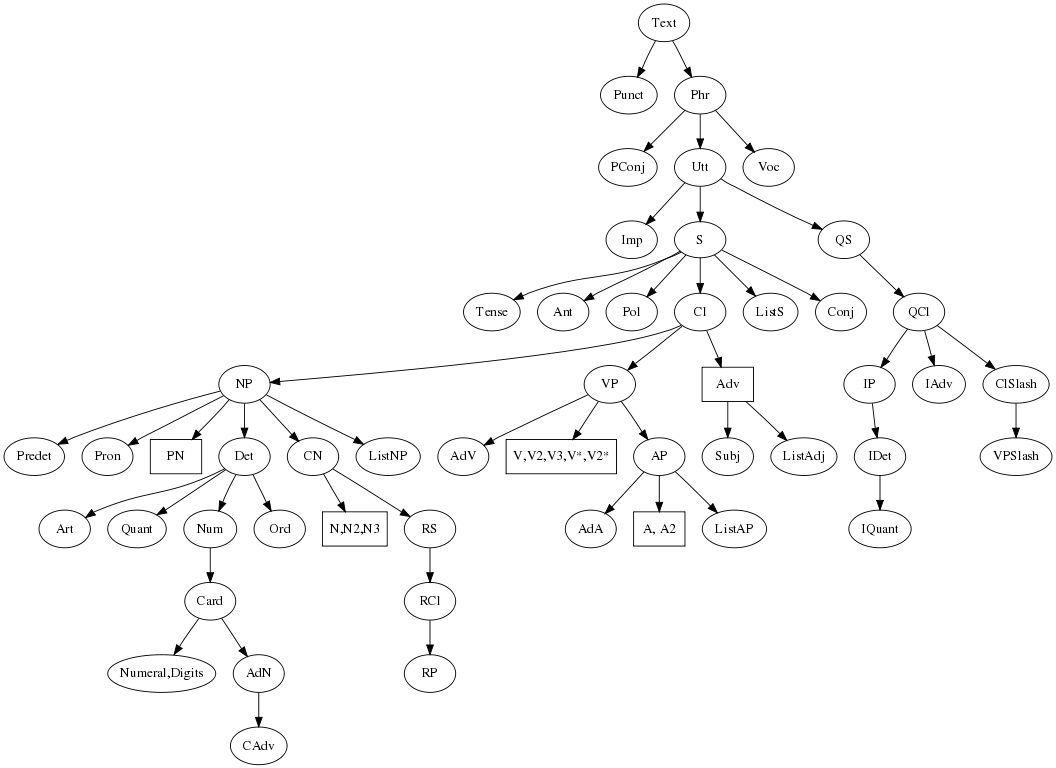
\includegraphics[height=130mm]{categories.png}
\caption{The types of the GF resource grammars. }
%TODO have footnote? where?
%\footnote{Available at http://www.grammaticalframework.org/lib/doc/synopsis.html}
\label{fig:gfpic}
\end{figure}

The concrete grammar gives a \textit{linearization type} for each category,
usually a record containing a table with the forms the word or phrase can be used in.
They may also
carry information about inherent features that matter to other parts of the sentence.

           
\newpage
\subsection{Noun phrases}
Section \ref{sec:writegf} contained an easy example with nouns. We used the categories \verb-N-
and \verb-N'- to distinguish nouns with respectively without number information.
%TODO read again
The category \verb-N'- was a simplification and is not used in the resource grammar. and is not used in the resource grammar.
The full analysis includes a distinction between the categories \verb-N- -- simple nouns --
and 
\verb-CN- -- common noun phrases -- and \verb-NP- -- noun phrases.
The \verb-N- category is implemented as an inflection table, generated by the smart paradigm,
and a field keeping information about the gender, see figure \ref{fig:gfflicka}.
\begin{figure}[h]
\begin{verbatim}
flicka_N = {s = {Sg Indef Nom =>  flicka
                 Sg Indef Gen =>  flickas
                 Sg Def Nom   => flickan
                 Sg Def Gen   => flickans
                 Pl Indef Nom => flickor
                 Pl Indef Gen => flickors
                 Pl Def Nom   => flickorna
                 Pl Def Gen   => flickornas ;
            g = utr }
\end{verbatim}
\caption{Representation of the noun `flicka' (\emph{`girl'}) in GF}
\label{fig:gfflicka}
\end{figure}\\
When a noun is turned into a \verb-CN- %, this information is kept, and the noun may
which may be modified by adjectival phrases or conjoined.
\begin{verbatim}
AdjCN : AP -> CN -> CN ; 
\end{verbatim}
The function \verb-DetCN-, determination, creates a
\verb-NP- by setting the number and definiteness of a \verb-CN-, shown in figure
\ref{gfcode:DetCN}.
%may be turned into a \verb-NP- by the rule \verb-DetNP- which sets
%the number and definitness.
%Since all morphological information is generated by the smart paradigms and contained in the \verb-N-
%the construction of a \verb-NP- more or less consists of putting the pieces together.
%The definitness is given by a determiner.

\begin{figure}[h]
\begin{verbatim}
DetCN : Det                  -> CN     -> NP ;
        indefinite, singular -> flicka -> "en flicka"
        definitive,singular  -> flicka -> "flickan"
\end{verbatim}        
\caption{}
\label{gfcode:DetCN}
\end{figure}
\newpage
%The two basic articles are \verb-IndefArt- and \verb-DefArt- which
%uses the post-modified form of the noun: katten.
Some rules for determination were described in section \ref{sec:swedishnoun};
if we have a common noun phrase consisting of the parts \emph{`liten'}
(\emph{`small'}) and \emph{`katt'} (\emph{`cat'}), there are three ways they
can be combined, as shown in figure \ref{tab:detdef}
\begin{figure}[h]
\begin{tabular}{|lll|l|}
\hline
\textbf{Determiner} & \textbf{Adjective} & \textbf{Noun} & \textbf{DetSpecies}\\
\hline
en  &  liten $[${\sc -Def}$]$& katt   $[${\sc -Det}$]$& \textbf{ DIndef}\\
min &  lilla $[${\sc +Def}$]$& katt   $[${\sc -Det}$]$  & \textbf{ DDef Indef} \\
den &  lilla $[${\sc +Def}$]$& katten $[${\sc +Det}$]$& \textbf{ DDef Def} \\
\hline
\end{tabular}        
\caption{}\label{tab:detdef}
\end{figure}

%Which combination that shoud be used is decided by the determiner. Hence all
Hence, all determiners
in our grammar must keep information about which definiteness they require; the
\verb-DetSpecies- parameter is stored as an inherent 
feature of the determiner.
The resource grammar distinguishes between quantifiers, 
determiners \verb-Det- and predeterminers. Predeterminers modify \verb-NP-s
while the other to modifies \verb-CN-s. The differences are shown in table
\ref{tab:detquant}. 
\begin{figure}[h]
\begin{tabular}{l|lll}
                        &\textbf{Has number}& \textbf{Has definiteness}& Example  \\ 
\hline
\textbf{Predeterminers} & --  & --  & alla katter, all maten \\ 
\textbf{Quantifiers}&-- &\checkmark  & min katt, mina katter, *min katten \\ 
\textbf{Determiners}   &\checkmark &\checkmark & varje katt, *varje katten, *varje katter  \\ 
\end{tabular}
\caption{}\label{tab:detquant}
\end{figure}

The definite article is considered to be a quantifier, which has the forms
\emph{en} and \emph{ett} for singular. In plural it
is the either \emph{``de"} or nothing, cf. sentence (\ref{sent:trottkatt2}a) and
\ref{sent:trottkatt2}b.
\enumsentence{\begin{tabular}[t]{@{}*{9}{l@{\ }}}   %\begin{tabular}[t]{@{}*{lllllll}}
a. & Katten        &sov. &&b. &\textbf{Den}  &gamla & katten  &sov.\\
   &\emph{cat}\small\sc+def &\emph{slept}&& &\emph{the} & \emph{old} & \emph{cat}\small\sc+def &\emph{slept}\\
\end{tabular}}\label{sent:trottkatt2}

We need to know if the common noun phrase 
has been modified, that is, whether the function \verb_AdjCN_ has been used.
However, once a category has been formed, there is no longer any information available
about how it was put together. This is a result of the functional approach
of GF. Therefore, %that is, whether the function \verb|AdjCN| has been applied.
this information
has to be passed on by an inherent feature of the \verb-CN-, a flag set to tell
if the \verb-AdjCN- was applied.
\begin{figure}[h]
\begin{verbatim}
DetNP : Det              -> CN        -> NP ;
        definite, plural +  katt      =  katter
        definite, plural +  stor katt =  de stora katterna
\end{verbatim}        
\caption{}\label{gfcode:defmod}
\end{figure}

%Their record
%has a field storing the
%which may  are called \verb-DIndef-, \verb-DDef Indef- and \verb-DDef Def-. 
%Additionally, we need to make sure that sentences as 
%\ref{sent:trottkatt}a are not allowed.

%TODO review, verify
Due syntax oriented analysis in GF, the GF category for pronouns \verb-PN- only
contains personal pronouns.
Many words which are considered to be pronouns in other analyses, such as The Swedish
Academy Grammar \cite{SAG}, only exist in 3rd person and are 
classified differently in GF, usually as determiners or quantifiers.
%Only personal pronouns are of the type \verb-Pron-.
 %TODO
 % Adjectives? About weak - strong - indefinite..

%TODO
%>> compare NP to HPSG.
%>> CN may be different in other theories.



\subsection{Verb phrases}
In figure \ref{fig:gftree1} we saw the GF representation of the sentence ``Jag
ser katten". The verb `ser' (\emph{`see'}) takes one object: `katten'.
In GF, this can be seen on the type of the verb,
valency information
is encoded into the lexicon. Transitive verbs have the type \verb-V2-, ditransitive
\verb-V3- etc. There are types for verb which takes sentences (\verb-VS-) and
adjectival (\verb-VA-) complements.
The lexicon is therefore a very important part of the
grammar. 
\begin{verbatim}
see_V2 ; 
SlashV2a   : V2 -> VPSlash ;
ComplSlash : VPSlash -> NP -> VP ;
\end{verbatim}

The function \verb-SlashV2a- lets you create a \verb-VPSlash-. The name
\verb-SlashV2a- is inspired by categorical grammar and is a short
hand for \verb-VP \ NP- -- a verb phrase missing a
noun phrase..  When we combine the \verb-SlashVP- with the object we
get a complete verb phrase.
Both the verb and its complements are stored in the verb phrase category, \verb-VP-.
%A simple idea would let the \verb-VP- consist of one field where the verb and object are
%glued together. But we also want to be able to express sentencens like
%``Du ser inte mig" and ``Mig ser du inte", where the object is separated from the verb.
%TODO explain, diff from Gazdar
The \verb-VP- category resembles the Didrichsen's field model.
%it has multiple fields that may be put in the different orders.
There are fields
for negation, different types of adverbs, objects, the finite verb and an infinite verb.
The fields may in turn be tables showing the different forms of the component.\\

\begin{tabular}{|l|llllllll|}
\hline
& & &&\textbf{VP}& & & & \\
\textbf{VP field} && \sc finit& \sc neg& \sc adV & \sc inf& \sc comp& \sc obj& \sc adv \\
\hline
&\emph{(han)} & har &  inte&  alltid&  tänkt&  på&  henne&  så \\
\hline
\end{tabular}\\

\vspace{5mm}
The verb phrase fields are not put in their correct order until the tense and type
of clause is determined, ie. when a sentence is created.\\

Swedish verbs may take up to five arguments \cite[p. 53]{stymne}.
These may be prepositions, particles, reflexive object, indirect objects
and direct objects. 
\enumsentence{\shortex{7}
{Jag &tar& med &mig& den& till& honom}
{\emph{I} &\emph{take}&\emph{with} &\emph{me}& \emph{it}& \emph{to}& \emph{him}}
{`I bring it to him'}
\label{sent:tamed}}
The verb `ta' in sentence (\ref{sent:tamed}) takes one particle (\emph{med}),
one preposition (\emph{till}) and two objects: \emph{den} and \emph{honom}.

In a GF lexicon this verb is given the
category \verb-V3-, %classifing it as 
a \textit{three-place verb}, taking two objects.
The notion \verb-V3- is motivated by the formal translation: \verb-bring(I,it,him)-.\\
%these will be encoded in different ways.
Particles are given in the lexicon, as well as the prepositions that are
chosen by the verb.
The entry for `\emph{ta med}', as used in sentence (\ref{sent:tamed}), is
described as follows:
%, assuming that we already have an constant \verb-take_V- which produces the correct conjugation for ``ta":
\begin{verbatim}
ta_med_V3 = dirV3 (reflV (partV (take_V "med")) (mkPrep "till") ;
\end{verbatim}
%The category \verb-V3- tells us that the verb takes two objects, % (``den" and ``honom").
The function \verb-dirV3- creates a three-place verb, where the first object is direct and
the second is to be used with the preposition given as the last argument: `\emph{till}'.
\verb-reflV- shows that the verb always is used with a reflexive
pronoun and \verb-partV- gives the particle \emph{`med'}.
The fact that the chosen prepositions is attached to the verb in the lexicon
causes the parse tree visualization algorithm to group them together.
This is also the case for particles, cf. parse tree \ref{pic:tittapart}
and \ref{pic:tittapa}.
As already stated, the visualized parse trees is not a complete representation,
even if the verb phrases in the the visualizations look the same, the two cases
are treated and represented differently internally. The fronting of the
preposition, as in of sentence (\ref{sent:tittapa}a)., is accepted but
fronting of particles, as in \ref{sent:tittapa}b., is not.
%TODO use png to get correct size
\eenumsentence{
\item[a]\shortex{4}
{På &pojken& tittar& du.}
{\emph{on} &\emph{the boy}& \emph{look}& \emph{you}}
{`You look at the boy.'}
\item[b]\shortexnt{6}
{*På& när& du& springer& tittar& jag}
{\emph{~on}& \emph{when}& \emph{you}& \emph{run}& \emph{watch}& \emph{I}}
\label{sent:tittapa}}
\begin{figure}[h]
\subfloat[Verb with a chosen preposition]{\label{pic:tittapa}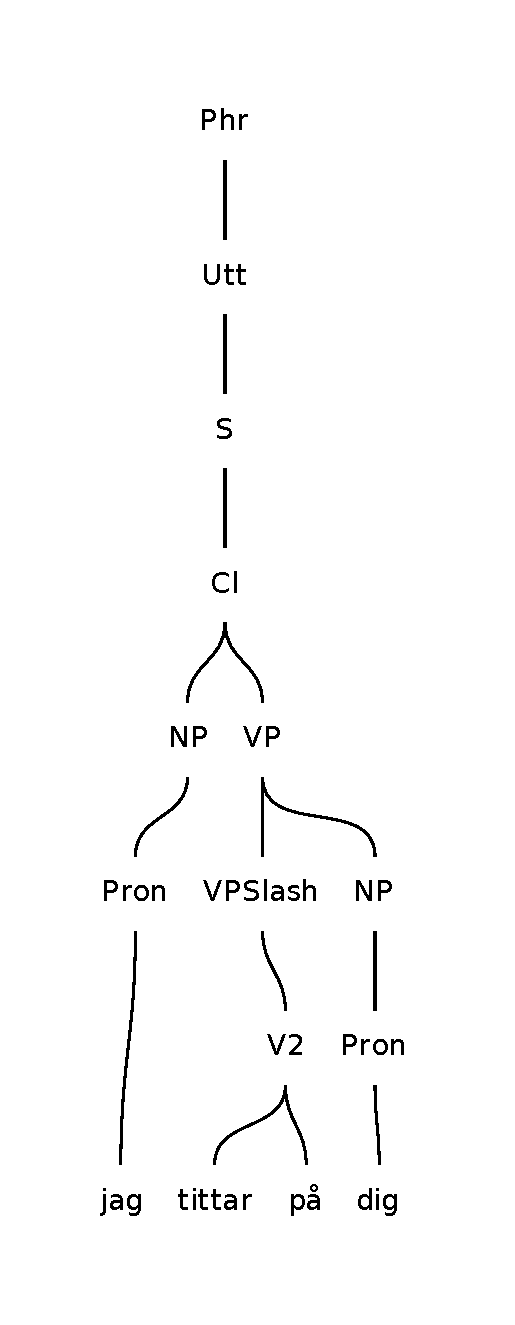
\includegraphics[height=80mm]{tittapa.jpg}}
\hspace{10mm}
\subfloat[Verb with particle]{\label{pic:tittapart}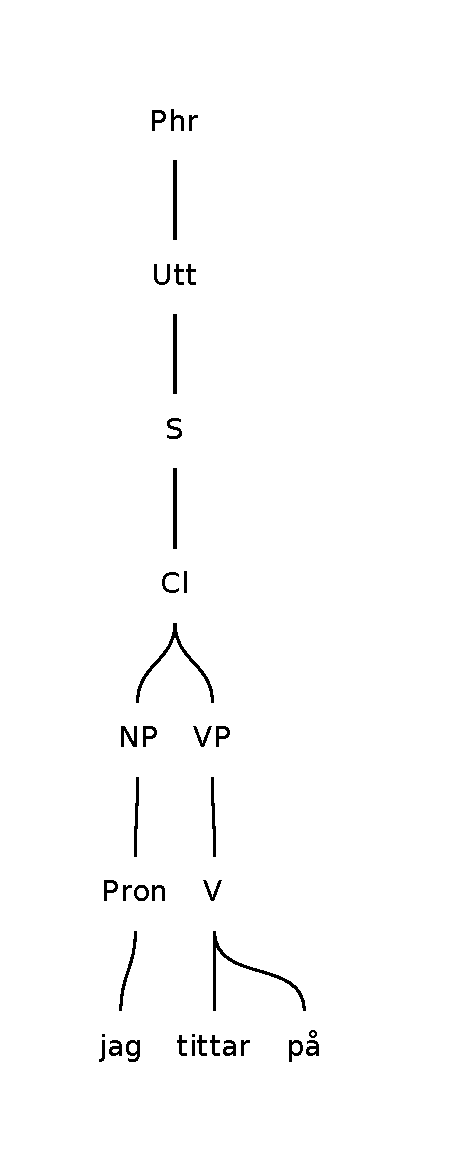
\includegraphics[height=80mm]{tittapart.pdf}}
\caption{The visualized parse trees do not show the internal difference of chosen prepositions and particles}
\label{fig:translationtrees}
\end{figure}


\newpage
%Categories as V,V2,VS...
%Maybe talk about ställa.
\subsection{Clauses}
The category clause, \verb-Cl-, represents a pre-sentence, that does not yet have any tense, polarity
or word order set, see figure \ref{fig:clause}.\\

\begin{figure}[h]
\begin{tabular}{|lll|ll|}
\hline
\textbf{Tense} &\textbf{Polarity} &\textbf{Word order} &\textbf{Cl} &\textbf{S} \\
\hline
present &negative & main        & du ser mig & 'Du ser inte mig'\\
perfect &positive & inverted    & du ser mig & 'Har du sett mig'\\
perfect &negative & subordinate & du ser mig & 'Du har sett mig'\\
\hline
\end{tabular}
\caption{}
\label{fig:clause}
\end{figure}


Like verb phrases, a clause may also be missing an object and then has the type
\verb-ClSlash-.
The \verb-ClSlash- is formed by a \verb-VPSlash- which is given a subject.
This is a convenient way to form questions, relative clauses
and topicalized clauses, as introduced by \cite{gazdar} (see figure \ref{fig:clause2}).\\

\begin{figure}[h]
\begin{tabular}{|l|ll|}
\hline
\textbf{Cl}& Johan + tittar på \\
\hline
\textbf{Wh-Questions} & Interrogative pronoun   & Vad tittar Johan på?\\
\textbf{Relative clauses} & Object + Relative pronoun & Katten som Johan tittar på \\
\textbf{Topicalized clauses} & Object  & Henne tittar Johan på \\
\hline
\end{tabular}
\caption{}
\label{fig:clause2}
\end{figure}


%
%Verbs with particles or verbs that choose a special  
%Particles and prepositions, can't be seen on the trees. Can now see why the parse
%trees are not complete. difference shows when fronting.
%tycka om /tycka om -> om vad tycker du inte. fast bra
%Swedish verb may have up to five arguments according to Stymne
%'jag tar med mig den till Bo' : 
%but is really 'till' part of verb?
%VP is divided corresponding to satsschema (diderichsen) (renewed by SAG).
%If the object is not given immediatly, the grammar uses slash.
%"Speed up", instead of movement used slashes \cite{gazdar}.
%Slashes good for question (vilken katt ser du idag)
%relatives (katten som du tittar på) and topicalisation
%The grammar has VP,Cl, SSlash, all missing NP.
%

%In some special cases, phrase cannot be put in all forms. 
%Give a good example!!
%It is not quite clear how to handle this at the moment. When
%the grammar is meant for parsing only, it is feasible to put
%a \textit{nonexist} pattern.
%example with this.\\

\subsection{Overview}
\vspace{4mm}
The original resource grammar could express complex sentences
as the one in figure \ref{gfSwe:parsetree}.
%shows the parse tree for sentence 
%\ref{gfSwe:parseable}.\\


%\enumsentence{\shortexnt{8}
%{Har& han& inte& ätit& de & gula& äpplena& idag?}
%{Has& he& not& eaten& the& yellow& apples& today?}} 
%\label{gfSwe:parseable}
%Covers sentences like
% better sentence where the verb phrase is split up?
\begin{figure}[h]
\includegraphics[width=70mm,height=70mm]{apples1.pdf}
\caption{Parse tree for ``Har han inte ätit de gula äpplena idag?"}
\label{gfSwe:parsetree}
\end{figure}
Even though the verb phrase \emph{``har inte ätit de gula äpplena idag"} is discontinuous, the whole
phrase is still treated as one constituent in GF. The parts
are connected in the tree, and the subject \emph{``han"} is put between the
finite verb and the rest of the phrase.
At the code level, This is done by putting the \verb-VP- fields in the correct order\\
\verb|table { Inv => verb.fin ++ subj ++ verb.neg ++ verb.inf ++ verb.compl ; ... | \\
%At the code level, this is implemented %using records.
%The linearization rule for questions -- clauses with inverted order -- picks 
%the field for the finite verb and appends it to the subject followed by
%the negation, infinite part and the complement of the verb phrase: \\

The resource grammar also covered relative clauses: 
\eenumsentence{\item[a]\shortexnt{5}{Hon & ser & pojken & som  &sover}
              {\emph{she} & \emph{sees} & \emph{the boy} & \emph{that} & \emph{sleeps}}
              %{`She sees the sleeping boy'}}
\item[b]\shortexnt{6}{Han & ser &katten & han  &tycker & om}
              {\emph{he} & \emph{sees} & \emph{the cat} & \emph{he} & \emph{likes} &}}
              %{`She sees the sleeping boy'}}

In addition to the core resource grammars, which is shared with the other languages implemented in the
library, 
%In addition to the basic resource grammar,
 language specific constructions may bee added
%>> core is shared but particular lang. has particular features.
to the module \verb|Extra|. The functions given here do not have to be translatable
to all other language, but are meant to cover language specific constructions.
Among those were functions for topicalisation: %$ although not all
%of them were implemented for Swedish.
%word order, agreement, tempus, adverbs, adjectivs...
%and relatives
%Also info in the Extra module, where more language specific constructions
%can be found.
%For example, \verb|FocObj| fronted the object as in sentence (\ref{gfSwe:apple}).
\enumsentence{\shortex{6}
{Det & äpplet & vill & jag & inte & ha}
{that & apple & want & I & not &have}
{`I don't want that apple'}}\label{gfSwe:apple}
and for preposition stranding:
\enumsentence{
~~Stranded preposition \hspace{45mm} cf.\\
\begin{tabular}{ll}
{\begin{tabular}{llllll}
Vem& måste& jag& akta& mig &\textbf{för}? \\
\emph{who}& \emph{must}& \emph{I}& \emph{watch out}& \emph{me} &\textbf{\emph{for}}? \\
\end{tabular}}&
{\begin{tabular}{llllll}
\textbf{För}& vem& måste& jag& akta& mig?\\
\emph{\textbf}{for}& \emph{who}& \emph{must}& \emph{I}& \emph{watch out}& \emph{me}?\\
\end{tabular}}\\
~~`Who do I need to watch out \textbf{for}?' &~ `\textbf{For} whom do I need to watch out?'\\
\end{tabular}}

%jag ser dig
%dig ser jag
%dig har jag inte sett
%jag har inte sett dig.
%how the parse tree is generated, the finite verb, the subject, the rest. usw.

%honom ville hon inte tänka på.



%What was in the resources
%description of the existing grammar, the types, the possibilities
%VP, NP.
%valency built in (problems with ställa - på, under, vid).
%Variants, nonexist.
%coverage of standard Swedish.

\section{Development of the grammar}
\label{sec:Added}
%The resource grammar is meant to cover the most important grammatical structures
%present in many languages, but not the language specific constructions.
It has earlier been hard to identify missing constructions of the Swedish
implementation, since there was no large resource available to evaluate it on.

Our evaluations are based on Talbanken, and when first conducting tests,
 we found much room for improvement.
From the topics listed in section \ref{sec:swedish}, the post-nominal articles
and the verb-second property
were covered by the resource grammar, as well as the periphrastic passive and
a limited form of topicalisation. 
The other constructions have been added during this project.
%enough to be covered by the resources. The others have been added.
%We have increased this by adding language specific
%constructions. Talbanken has been our inspiration.
%>> the grammar will not be totally covering, but interesting and useful.
%>> hard to estimate before, since no big use case/resource.
%>> after initial experiments, first evaluation. found much room for improvement. 
%>> discovered constructions missing.

%%PASSIV
\subsection{The s-passive}
Passive voice is often used in Swedish, especially the
\textit{s-passive}.
\enumsentence{
\shortex{5}{Uppsatsen & skrev\textbf{s} & av & en & student.}
        {\emph{the essay} & \emph{wrote+\textbf{s}} & \emph{by} & \emph{a} & \emph{student}}
        {`The essay was written by a student.'}}\label{sent:skrevs}
%{b. &En & student & skrev & uppsatsen.}
%        {&a &student &wrote &the essay}
%        {~~`A student wrote the essay.'}}
Some studies suggest that the s-passive is used in more than 80 \% of the times
\cite{laanemets}.
It is however not as common in the other Scandinavian languages, 
where not all words have passive forms for all tenses. The Norwegian 
translation of sentence (\ref{sent:skrevs}) is:
%The periphrastic passive is preferred, especially in spoken langauge.
\enumsentence{\shortexnt{7} %\begin{tabular}{ll}
{Oppgaven &ble& skrevet& av& en& student & [NO]}
{uppsatsen& blev& skriven& av& en & student& [SE]}}
%\end{tabular}}
The corresponding Swedish sentence is acceptable, but not as natural sounding as sentence
(\ref{sent:skrevs}).
The resource grammar for Scandinavian therefore implemented the function for passive,
\verb-PassV2-, by using auxiliary verb. \\
\begin{verbatim}
PassV2 : V2  -> VP ;
         ta -> blev tagen
\end{verbatim}
%>> how are they used with reflexives??
The function allows two-place verbs to be used in passive by using \emph{bli} (\emph{become}), and thereby
turned into complete verb phrases; they no longer need an object.\\

During this project, the s-passive was added as the standard case.
Periphrastic passive is still allowed, but as an alternative rather
than the default.
The grammar further allows not only V2, but all verb phrases that misses an object, to 
form passives:
\begin{verbatim}
PassVP : VPSlash -> VP ;
         ta      -> togs
         erbjöd  -> erbjöds
\end{verbatim}
A \verb-V3- like `give' in sentence (\ref{sent:give2pass}) gives rise to two
passives, (\ref{ex:passV32}) and (\ref{ex:passV33}).
\enumsentence{\textbf{Active use of two-place verb}\\\shortex{4}
{Vi & erbjöd& henne& jobbet }
{\emph{we} & \emph{offered}& her&\emph{the job}}
{`We offered her the job'}}
\label{sent:give2pass}
\enumsentence{\textbf{First place in two-place verbs}\\\shortex{3}
{Jobbet & erbjöds & henne }
{\emph{the job} & \emph{offered+\textbf{s}}&\emph{ her}}
{`The job was offered to her'}}
\label{ex:passV32}
\enumsentence{\textbf{Second place in two-place verbs}\\\shortex{3}
{Hon & erbjöds & jobbet}
{\emph{she} &\emph{ offered+\textbf{s}}&\emph{ the job}}
{`She was offered the job'}}
\label{ex:passV33}
\enumsentence{\textbf{V2A verb}\\\shortex{3}
{Huset & målades & rött}
{\emph{the house} & \emph{painted+\textbf{s}}& \emph{red}}
{``The house was painted red"}}
\label{ex:passV2A}

\subsection{Impersonal constructions}%Presentering, , Topicalisering
\label{sec:Formal}
Formal subjects \cite[\textsection 19]{SAG} are often used in Swedish.
\enumsentence{\shortex{6}
{Det & sitter & en & fågel & på & taket}
{\emph{it }& \emph{sits }& \emph{a} & \emph{bird} &\emph{ on} & \emph{the roof}}
{``There is a bird sitting on the roof''}}
\emph{`Det'} has the position of the subject, and the real subject, 
\emph{`en fågel'} the one of an object.

Transitive verbs may not be used like this
\enumsentence{\shortexnt{7}
{*Det & äter & en & fågel & frön & på & taket}
{~\emph{it} & \emph{eats} & \emph{a} & \emph{bird} & \emph{seeds} & \emph{on }& \emph{the roof}}}
\label{sent:fagelfron}

unless their in passive form
\enumsentence{\shortex{5}
{Det&dricks&mycket & öl& nuförtiden}
{\emph{It}&\emph{drink+s}&\emph{much} &\emph{ beer}&\emph{ nowadays}}
{``A lot of beer is being drunk these days"}}
A very common example of this is sentences with the verbs \emph{finnas},
(\emph{exist})
\emph{saknas} (\emph{miss}) and \emph{fattas}(\emph{lack}).
\enumsentence{\begin{tabular}[t]{@{}*{14}{l@{\ }}}
a. &Det & finns & kaffe &
b. &Det & saknas&  kaffe &
c. &Det & fattas & kaffe \\
&\emph{it }& \emph{exist }& \emph{coffee} &
 &\emph{it }& \emph{misses} & \emph{coffee} &
 &\emph{it} & \emph{lacks} & \emph{coffee}\\
\end{tabular}\\
{~~''There is coffee"~~ ''There is no coffee"~~ ''There is no coffee"}}


To implement this construction, we needed a
special GF category, \verb|SimpleVP|, to exclude other verb phrases
like the one in sentence (\ref{sent:fagelfron}). Any intransitive verb can form
a \verb-SimpleVP-, as can transitive verbs without their objects. The \verb-SimpleVP-
may be modified by adverbs.

There are also restrictions on the real subject, which is not allowed to be in
definite form.
\enumsentence{\shortexnt{6}
{*Det     & sitter     & \textbf{den}& \textbf{fågeln}& på       & taket.}
%& *Det sitter \textbf{fågeln} på taket.\\
{\emph{it}& \emph{sits}& \emph{the}  & \emph{bird}    & \emph{on}& \emph{the roof}}
%& ``There are the bird sitting on the roof'' \\
}
Neither is sentence (\ref{sent:dumfagel}) correct.
\enumsentence{\shortexnt{6}
{*Det& sitter& \textbf{min}& \textbf{fågel}& på& taket}
{\emph{it}&\emph{sits}&\emph{my}&\emph{bird}&\emph{on}&\emph{the roof}}
%``There are my bird sitting %on the roof''\\
}\label{sent:dumfagel}
In order to implement this, we utilized the 
%The distinction lays in the determiner. The
different types of determiners shown in figure \ref{tab:detdef}. 
For postverbal subjects, the determiner must be of type \verb-DIndef-,
that requires both the noun and the adjective to be indefinite.
%The quantifier must have determiner must havenoun must be in indefinite form,
%even though some determiners are allowed.
%\enumsentence{\begin{tabular}[t]{@{}*{5}{l@{\ }}}
%a. & Det sitter några fåglar på taket    & & b. & Det sitter fåglarna på taket\\
%   & ``There are some birds on the roof''& &    & ``There are the birds on the roof''\\
%\end{tabular}}\label{sent:faglar}
%Sentence \ref{sent:gamlafagel}b exemplifies a determiner that uses the noun in indefinite form,
%but the adjective in definite form.
%\enumsentence{\begin{tabular}[t]{@{}*{5}{l@{\ }}}
%a. & Det sitter en gammal fågel på taket.& & b. & * Det sitter min gamla fågel på taket.\\
%   & ``There are some birds on the roof''& &    &~ ``There is my old bird on the roof.''\\
%\end{tabular}}\label{sent:gamlafagel}
%
%%Quantifiers like \emph{`denna'} or determiners like \emph{`samtliga'} may
%%not be used, but the determiners \emph{`många'}, \emph{`några'} and the quantifier
%%\emph{`ingen'} work well.
%%Semantic difference, atm we allow any NP. \\
To form a clause with formal subject, we hence need to inspect the determiner.
\begin{verbatim}
FormalSub : SimpleVP -> Det -> CN -> Cl ;
\end{verbatim}
The function combines a verb phrase, a determiner and a noun phrase to a clause.
If the determiner does not fulfill the requirements stated above, the clause is
put to NONEXIST.
This works well for parsing, but leads to problems if the grammar is used
for random generation. The solution is thus not ideal,
but since the definiteness of noun phrases or determiners cannot be seen on the
type level, it is not known until runtime whether the determiner is accepted
in the subject.

% move to future?
As a future direction it would be interesting to examine the consequences of
letting the noun phrases have more information on the type level. In the
implementation for reflexive objects  (see section \ref{sec:reflexives}),
dependent types are used for showing if a noun phrase 
needs an antecedent.
We would also like to differentiate between the \verb-NP-s in sentence
(\ref{sent:mosthorses}a,b), where 
`\emph{av}' should be used
only when the noun has an explicit article or determiner.
\enumsentence{\begin{tabular}[t]{@{}*{5}{l@{\ }}}
a. &De flesta hästarna  && b.& De flesta \textbf{av} de där hästarna.\\
 &``Most of the horses"  && b.&  ``Most of those horses."\\
\end{tabular}}\label{sent:mosthorses}

%There are other examples of when we need to know the definiteness of the noun phrase 
%%, for example when using %the reflexive possessive pronoun `sin' (see section `Reflexive pronouns' below)
%or when using some predeterminers (see section `Quantifiers'). Not true, not the same :(

%finnas: här får man ha definit: det finns de som inte vill. Samma RelCl som
%jag just la till, de äppplen. (de + relsats)

%'det är kul att..' Näst vanligaste två-ordskombinationen i talad svenska.
%%
%embedded - relative, 'sådan att' not really nice for normal swedish, and no agreement
%between subject 'en katt sådan att det regnar'. Kan säga 'en sån katt som sover, med 'sådan' + Rel
%har lagt till Det äpple + Rel (RelCNNP). *Det äpple är rött. men Det äpple jag äter är rött.
% 
\subsection{Formalizing the rules for reflexive pronouns by using dependent types}
\label{sec:reflexives}
An important area in a Swedish grammar is the treatment of the reflexive pronouns and
%TODO fix page ref
the reflexive possessive pronouns as described on p. \pageref{swe:refl}.
The reflexives require an antecedent with which they agree in
number and person.
Our grammar should accept the following sentences:

\enumsentence{Han såg sina barns skor.\\ \label{ex:ReflGen}
He saw {\sc self's} children's shoes.}
\enumsentence{Sina vantar hade han glömt på tåget.\\
{\sc self's} gloves, he had forgotten on the train.}
%\enumsentence{Han ger sina pengar till sina syskon.\\
%He gives {\sc self's} money to {\sc self's} children.}
\enumsentence{Hon ber alla sina kompisar att gå\\
She asks all {\sc self's} friends to leave}\label{ex:ReflPredet}
\enumsentence{Jag vill att han rakar sig.\\
I want him to shave {\sc self}.}
\enumsentence{\begin{tabular}[t]{@{}*{5}{l@{\ }}} 
a. & Han är längre än sin kompis. & & b. &Han är här oftare än sin kompis.\\
   & He is taller than {\sc self's} friend.
   & & & He is here more often than {\sc self's} friend.
\end{tabular}}\label{ex:ReflAP} \label{ex:ReflAdv}
\eenumsentence{%\begin{tabular}[t]{@{}*{5}{l@{\ }}}
\item Hon tyckte om skolan och alla sina elever.\\
     She liked the school and all {\sc self's} students.
\item Han såg sina få böcker och sin penna.\\
 He saw {\sc self's} few books and {\sc self's} pencil.
}\label{ex:ReflConj} \label{ex:ReflConj2}
Reflexive pronouns can not be used in subject noun phrases of finite sentences,
as shown by the ungrammatical examples in %, it is hence not
%allowed as subject. The antecedent must not be out of scope for the closest finite verb,
sentence (\ref{sent:sesig}) and (\ref{ex:ReflSubj}).
The third person reflexives (`sig',`sin') requires a third person antecedent (see \ref{ex:refljag}).
Furthermore, the antecedent must be within the same finite sentence as the reflexive
pronoun, see (\ref{sent:sesig}).
The grammar should not accept any of these sentences:
\enumsentence{
*Sina vantar var kvar på tåget.\\
{\sc self's} gloves were left on the train.}\label{ex:ReflSubj}
\enumsentence{*Hon och sin kompis läser en bok.\\
She and {\sc self's} friend are reading a book. }
\enumsentence{*Jag ger sina pengar till sina syskon.\\
I give {\sc self's} money to {\sc self's} siblings. }\label{ex:refljag}
\enumsentence{*Han vill att jag ser på sig.\\
He wants me to look at {\sc self}.}\label{sent:sesig}

Apart from these restrictions, noun phrases containing reflexive pronouns
may be used as any other \verb-NP-. They may be conjoined 
(\ref{ex:ReflConj} a,b) and used with other determiners (\ref{ex:ReflPredet}).
In the standard GF analysis, which is preformed bottom-up starting from the pos-tags, 
all information about semantical roles are lost. There is no way
of knowing whether a \verb-NP- acts as subject or object. For this reason,
the formalization of reflexive pronouns required the use of a different analysis.
%and used as genitives (sentence \ref{ex:ReflGen}) as such.
%Could be combined with 'sig', a ReflNP without another noun.
In short, what is wanted can be summarized as follows:\\
%\begin{figure}[h]
\begin{enumerate}
\item{
Construct a noun phrase from a common noun phrase \\
katt $\rightarrow$ sin katt} % \\
\item{Modify it like a \verb|NP|\\
sina katter $\rightarrow$ alla sina katter}
\item{Use it only as object\\
sin katt $\rightarrow$ han såg sin katt }
\end{enumerate}
%\caption{Rules for noun phrases with reflexive possessive pronouns}
%\label{fig:reflrestrict}
%\end{figure}


If we ignore the second requirement, we might come up with a solution where
special functions for using common nouns
together with reflexive possessive pronouns are introduced:
\begin{verbatim}
ReflVP: CN -> VPSlash -> VP ;
        mat + äta     -> äta sin mat 
\end{verbatim}
This way, using the phrases as subject is excluded, but none of sentence
(\ref{ex:ReflConj} a,b) or (\ref{ex:ReflPredet}) are allowed.\\
The simplest way to fix this is to treat the phrases as normal \verb_NP_s.
We can add a rule that allows using the possessives with common noun phrases:
\begin{verbatim}
ReflNP: CN -> NP ;
        mat -> sin mat 
\end{verbatim}
They may now be used with predeterminers:
\begin{verbatim}
PredetNP : Predet -> NP       -> NP ;
           alla   + sina barn -> alla sina barn
\end{verbatim}
But by keeping them as \verb_NP_s we lose information, and there is no way of
keeping them from being used as subjects. We have ignored the third restriction
and the grammar would generate and accept sentence (\ref{ex:ReflSubj}).

We get closer to a satisfying solution by introducing new object type,
\verb_Obj_, which is
identical to normal \verb_NP_ except that it depends on 
the antecedent. All functions where objects are modified in the same way
as other \verb-NP-s are duplicated, one version is dealing 
with objects and one with \verb-NP-.
\begin{verbatim}
ReflVP: Obj     -> VPSlash -> VP ;
     -- sin mat +  äta     -> äta sin mat 
NPtoObj : NP  -> Obj ;
PredVP  : NP -> VP -> Cl ;  -- NP used as subject
\end{verbatim}
Any normal noun phrase may also be used as an object, whereas subjects only
can be made up by \verb-NP-s.
The drawback of this solution is the duplication of functions.
\begin{verbatim}
PredetNP  : Det -> NP  -> NP ;
PredetObj : Det -> Obj -> Obj ;
\end{verbatim}
%We will need functions for conjugating objects with objects, 
% say smt about overgeneration?
The dependence on the antecedent needs to be applied to adverbial phrases and
adjective phrases as well. The adjective phrase in (\ref{ex:ReflAP}a) and
the adverbial phrase in (\ref{ex:ReflAdv}b) are examples of this; if the
subject was changed to 2nd person, they  would need to change too.
\enumsentence{\begin{tabular}[t]{@{}*{5}{l@{\ }}} 
a. &\textbf{Du} är längre än \textbf{din} kompis.& b. &*Du är här oftare än \textbf{sin} kompis.\\
 & You are taller than your friend. &&You are here more often than {\sc self's} friend.\\
\end{tabular}} \label{ex:ReflAP2} \label{ex:ReflAdv2}
The dependency spreads through the grammar and in order to avoid all code
duplication we use another approach.
When looking at the type of
the functions, we notice that they can be generalized:
\begin{verbatim}
PredetNP  : Det -> NP x  -> NP x;
\end{verbatim}
The solution chosen in this project is to make use of this generalization and
introduce the use of dependent types in a resource grammar.
Following the idea given above, we make a difference between subjects and objects, but not
by giving them different types, but by % treating them as instances of the \verb-NP- category.
letting the type \verb-NP- \textit{depend} on an argument, which may either be \verb-Subject- or
\verb-Object-.
\begin{verbatim}
cat NP Boolean ;
PredVP     : NP Obj  -> VP     -> Cl ;
ComplSlash : VPSlash -> NP Obj -> VP ;
PredetNP   : (a : Boolean) -> Det -> NP a -> NP a ;
\end{verbatim}
The types for adverbial and adjectival phrases are also turned into dependent
types.
\enumsentence{\shortex{3}
{taket & på sitt hus &}
{\scriptsize{\textbf{NP a +}} & \scriptsize{\textbf{(Adv Obj)}} & $\Rightarrow$ \scriptsize{\textbf{NP Obj}} }
{\emph{the roof of {\sc self's} house}}}
%{{\sc NP +} & {\sc (Adv with Obj)} & $\Rightarrow$ {\sc Obj}}
\enumsentence{\shortex{3}
{sitt hus & på berget &}
{\scriptsize{\textbf{NP Obj + }} & \scriptsize{\textbf{Adv a}} & $\Rightarrow$ \scriptsize{\textbf{NP Obj}} }
{\emph{{\sc self's} house on the mountain}}}


We hence combine the-part-of-speech driven analyse normally preformed by
GF with a part-of-sentence analysis, where the dependent types gives the semantical
information we were missing.

The use of dependent types separates our grammar from the other resource grammars. Such separation
is not desirable in itself, but there are at least two reasons why we
believe it is appropriate in this case:
\begin{itemize}
\item The new grammar can be made compatible with the old implementation.
%TODO verify
\item The possibility for noun phrases to agree with an antecedent 
      will be useful in other languages. For example, the Slavic and Romance languages
      have similar reflexive pronouns.
\end{itemize}
Moreover, the goal of the project is to make a language specific grammar, and it
would be surprising if this could be done while leaving the abstract grammar unchanged.

Dependent types are also interesting for other problems.
The rules for reciprocal pronouns could be formalized using the same idea. As
reflexive pronouns, reciprocals (sentence \ref{sent:varandra})
must not be used as subjects and furthermore they may only be used when the
number of the antecedent is plural.
\enumsentence{
\shortex{3}
{De &ser& varandra}
{\emph{they} &\emph{see}& \emph{each other}}
{`They see each other'}}\label{sent:varandra}
%\item \shortexnt{3}
%{*Han &ser& varandra}
%{~he &sees& each other}}
%
%Since the resource grammar did not make any distinction between
%
%subjects and objects, the new Swedish grammar needed to be separated from the old
%structure. 
%The first restriction in figure \ref{fig:reflrestrict} should be slightly
%modified, to allow certain kind of \verb|NP|s to be used.
%\begin{figure}[h]
%\begin{enumerate}
%\item{
%Construct a noun phrase from a common noun phrase or certain noun phrases \\
%få katter $\rightarrow$ sina få katter} 
%\end{enumerate}
%\caption{Modification of \ref{fig:reflrestrict}}
%\end{figure}
%
%The kind of noun phrases that can be used seems to coincide with the ones
%that can be used with formal subjects (see section `Impersonal constructions').
%>> subject controlling verbs
%>> why comlicated with doubled types, show simplicity (elegant) with dep.types, and
%>> some problems (many fields).
%>> samesame as Obj, but conjunction works too, sin is Quant but what i sig?
%>> (show circle (sig : NP -> GenNP sig -> sin??)
%>> how we can add dependent type for Num to use 'varandra'
%>> CN should have dettyp too, 'avståndet till sin bil'
%\verb- PhrUtt NoPConj (UttQS (UseQCl (TTAnt TPres ASimul) PPos (QuestVP whatSg_IP (ComplSlash (NPObj ?10 (DetCN ?10 (DetQuant ?10 (IndefArt ?10) NumSg) (UseN woman_N))) (SlashV2a fight_V2))))) NoVoc-
%  ajaj unknown here!!

%>>Mention varandra. Same idea.
%>>agreement to subj: Also good for double functions : Flickan, hon var inte dum, hon?
% F1,2,3 : NP -> VP -> Cl ; NP needs gender (Masc,Fem,Utr,Neutr)


%Make a distinction between objects and subjects?
%do not want to copy all rules for another category. Would like depent types!
%work pretty well by letting all NP depend on the subject in the phrase.
%The current version is nice and works for recursive genitivs!
%Extra info, but maybe this is just the case about NPs.
%Discuss how other solutions, NPR and Predet : Predet -> CN -> NPR ;
%*Slash* : VPSlash -> NPR -> VP ;
%Keep number of fields down, but introduces another category, and one more
%label to the parse tree, is it interesting? How to combine it with genitive 
%without making it ambiguous (Han såg barnens hund).
%What if we add alot of other rules that uses NP, will they all need to be
%duplicated then?

%'han såg sin mammas bil', they same could be applied to
%APs for example \ref{ex:ReflAP} or Adv for
%\enumsentence{Han leker oftare än sin kompis}
% (ComparAdvAdj)
%Atm you can't focus this kind of object, then a ClSlash need info about the
%subject. FunRP also tricky (and what does it mean, we can say
%Han såg sin katt i vilken musen låg), in this case RP needs to give more information.
%Kort sagt, the information about the subject must be spread
%in different parts of the sentence. 
%Could also decide to always produc 'sin' -> jag såg sin bil
%to avoid the dependence, but not nice. Or keep a flag in NP saying if it is
%in third person, and add nonexist for others. But this way we can also get rid
%of ReflVP and the possessive prons \verb|PossPron| should only be used for somebody else:
%'jag såg din bil'.
%Unfortunaly, have to change ReflVP, this only allows this in object for VPSlash, not FocObj,
%not 'alla sina', usw. Want it to handle conjuction as in example \ref{ex:refGen}
%etc.
%varandra, works the same but has no case for Sg.
%%

\subsection{A second future tense: ``Kommer att"}
Swedish and Norwegian use two auxiliary verbs for future tense
\cite[p. 246]{H&H}:
%\cite[Tempus \textsection 28]{SAG}.
\enumsentence{\begin{tabular}[t]{@{}*{5}{l@{\ }}}
a. & Det \textbf{kommer att} bli mörkt snart & & b. &Jag \textbf{ska} gå och lägga mig nu\\
  & ``It will get dark soon" & &  &``I'm going to bed now"\\
\end{tabular}}
\enumsentence{
Jeg kommer til å savne deg ~~$[$NO$]$\\
``I will miss you"}
The modal verb \emph{``ska"} signals an intention of committing the action, either from the subject or from
the speaker. Cf.
\enumsentence{\begin{tabular}[t]{@{}*{5}{l@{\ }}}
a. & Du ska tycka om den & & b. &Du kommer tycka om den\\
  & ``You \emph{shall} like it" & &  &``You will like it."\\
\end{tabular}}
The verb \emph{``kommer"}, normally used with the infinite marker \emph{att},
does not signal any intention, but that the speaker has belief that 
it will actually come true.\\
The resource grammar included 
\emph{``ska"}, which was implemented as the standard way of forming future
tense, and hence represents the translation of
\emph{``will"}. 
The new grammar also supports \emph{``kommer att"}, expressed as an alternative
future tense.
\begin{figure}[h]
\begin{verbatim}
(UseCl (TTAnt TFutKommer ASimul) PPos 
       (ImpersCl (AdvVP (ComplVA become_VA (PositA dark_A)) soon_Adv))
\end{verbatim}
\caption{Result of parsing ``Det kommer att bli mörkt snart". The future tense
         is marked by the constant TFutKommer}
  \label{fig:kommeratt}
\end{figure}

%since we believe it will happend, it can not be as in :
%'det ska (kommer*) bli fint väder imorn, men de kanske har fel'.
Since two out of the three Scandinavian languages share this
tense, it has been added to the Scandinavian \verb-Extra- module.
Table \ref{fig:kommeratt} shows how the grammar expresses new tense
in different types of sentences.
\begin{figure}[h]
\begin{verbatim}
s SFutKommer Simul Pos Main : jag kommer att se henne
s SFutKommer Simul Pos Inv  : kommer jag att se henne
s SFutKommer Simul Pos Sub  : jag kommer att se henne
s SFutKommer Simul Neg Main : jag kommer inte att se henne
s SFutKommer Simul Neg Inv  : kommer jag inte att se henne
s SFutKommer Simul Neg Sub  : jag inte kommer att se henne
s SFutKommer Anter Pos Main : jag kommer att ha sett henne
s SFutKommer Anter Pos Inv  : kommer jag att ha sett henne
s SFutKommer Anter Pos Sub  : jag kommer att ha sett henne
s SFutKommer Anter Neg Main : jag kommer inte att ha sett henne
s SFutKommer Anter Neg Inv  : kommer jag inte att ha sett henne
s SFutKommer Anter Neg Sub  : jag inte kommer att ha sett henne
\end{verbatim}
\caption{The covered and accepted usage of the future tense with `komma'}
  \label{fig:kommeratt}
\end{figure}

%r
%\enumsentence{\shortex{6}
%{Betyget & 3 &ges &till &många &elever}
%{Grade & 3 & give+\textbf{s}& to & many & students}
%{``Grade 3 is given to many students"}}
%\label{ex:passV3}
%by letting the first object be `removed' and given by the subject. 
%
%A remark can be made about sentences where the second object is put first in the sentence, like 
%\enumsentence{Till många elever ges betyget 3}
%This is a variant of example \ref{ex:passV3}, \emph{`många elever'} is still the object but put in focus. The grammar
%parse this by applying \verb|FocObj|.
%%
\subsection{Modifying verb phrases}
\subsubsection{Focusing adverbs}
The GF analysis distinguishes between two categories of adverbs: \verb-Adv- 
%e.g. `nu' (\emph{`now'}) and
and \verb-AdV-. %like `alltid' (\emph{`always'}).
The \verb-AdV- (e.g. `aldrig' (\emph{`never'}) and `inte' (\emph{`not'}))
attaches directly to the verb.
%and have a special field in the \verb-VP--table.
\enumsentence{Cf.\\\begin{tabular}[t]{@{}*{12}{l@{\ }}}
a. & Jag & äter & \textbf{aldrig} & fisk & & b. &Jag & äter & fisk& \textbf{nu}\\ 
&\emph{I} & \emph{eat} & \emph{never} & \emph{fish} &&&\emph{ I }&\emph{ eat} &
\emph{fish}& \emph{now}
\end{tabular}\\
``\hspace{1mm} I never eat fish" \hspace{9mm} ``I eat fish now"}
The difference is implemented by having separate fields in the \verb-VP- table
for the two categories.
\begin{verbatim}
Main clause : subj ++ verb.fin ++ verb.adV ++ verb.inf ++ verb.adv
              han     har         aldrig      varit       här 
\end{verbatim}
%\begin{wrapfigure}{l}{0.3\textwidth}
%\begin{tabular}{|l|}
%\hline
%bara \\
%inte ens \\
%till och med \\
%\hline
%\end{tabular}
%\caption{Focusing adverbs}
%\label{fig:focadv}
%\end{wrapfigure}\\
The adverb `bara' may be used as an \verb-AdV- but also before the finite verb,
when emphasizing the verb itself.
This is an example of a \textit{focusing adverb}, others examples are `inte ens' (\emph{`not even'})
and `till och med' (\emph{`even'}).
\enumsentence{\shortex{11}
{a. & Han & bara & log  && &b. & Hon& till och med& visslar}
{&\emph{he} & \emph{only} &\emph{ smiled} & & & &\emph{she} &\emph{even} & \emph{whistles}  }
{~~``He just smiled"\hspace{8mm} ``She even whistles"}}
Focusing adverbs are accepted by the new grammar implementation, where they have
their own field in the \verb-VP-table.
\begin{verbatim}
Main clause : subj ++ verb.focAdv ++ verb.fin ++ verb.adV ++ verb.inf ++ verb.adv
              han     bara           sover        -             -           -
\end{verbatim}
They may also be used as \verb-AdV-...
\enumsentence{\shortexnt{4}
{Han & har & bara  & sovit}
{\emph{he} & \emph{has} & \emph{only}  &\emph{ slept}}}

...or as predeterminers:
\enumsentence{\shortex{8}
{Det & är & bara & barn &som& får & göra & så }
{\emph{it} & \emph{is} & \emph{only} & \emph{children} &\emph{that}& \emph{may} & \emph{do} & \emph{so} }
{`Only children are allowed to do that'}}
Two more rules are consequently needed
\begin{verbatim}
FocAdvAdV : FocAdv -> AdV ;
PredetAdvF : AdvFoc -> Predet ;
\end{verbatim}



The focusing adverbs are usually not combined with modal verbs, the copula or temporal auxiliaries. 
% since the modal verbs rarely are focused.
\eenumsentence{\item[a]
\shortexnt{5}
{?&Han & bara&  är&  dum}
{&\emph{he} &\emph{ only} & \emph{ is}& \emph{ stupid}}
\item[b]
\shortexnt{5}
{?&Han & bara&  har&  sovit}
{&\emph{he} &\emph{ only} & \emph{ has}& \emph{ slept}}}
We have however chosen to allow this, since it is grammatically correct although semantically
dubious, and since \emph{``Han har bara sovit"} is covered by the rules using focusing
adverbs as \verb-AdV-.
%The semantic aspect of focusing adverbs remains rather unclear in this
%representation. 
%Discussion: should han åt bara ett äpple be (bara ett äpple) focusing an NP?
%Then what about: han har bara sovit, han har bara ätit ett äpple.\\

%Ask elisbet for other examples with inte ens och till och med, nätt och jämt.
%In order to implement this, a new field was needed in the \verb-VP--table,
%which may be put before the finite verb.\\
%\verb|s SPres Simul Pos Main : han bara sover|\\
%compare to negation, \verb-AdV- and \verb-Adv-\\
%\verb|s SPres Simul Neg Main : han bara sover inte alltid här|\\
%example in Sub or Inv, 
%When used together with modal verbs, the new field results in
%some not very natural sounding constructions:\\
%\verb|s SPres Anter Pos Main : han bara har sovit|\\
%but rather than changing to 'han har bara sovit', we keep it. Is a possible
%tolkning and the other case is covered by using it as an AdV, we don't want
%ambiguities.
%\subsubsection{PPartAP}
%The VP require many changes PPart, bara.

%PPartAP : V2 -> AP ; --VPSlash -> AP ;
%
%About PPart, but do we need it with new Saldo? 'de är stuckna' , 'den nyligen
%funna'
%for the last one, we need VPSlash to allow adverb.

\newpage
\subsection{Miscellaneous}
This section covers some minor changes of the grammar.
They are described
as documentation of the implementation, and to illustrate some problems
and solution of more general nature.
\subsubsection{Relative clauses}
The resource grammar already gave a good coverage of relative clauses and embedded sentences.
All constructions used in examples \ref{sent:relex}a-d were accepted.
%provided a number of ways to express relative and embedded clauses, such as
\eenumsentence{
%\item[a.]Frågan är vilken färg den har
\item[a.]Pojken, som är blyg, tystnar\\
`The boy, who is shy, falls silent'
\item[b.]Han såg kunden som tyckte om sallad\\
`He saw the customer who liked salad'
\item[c.]Jag tänkte på huset i vilket hon bodde\\
`I thought about the house in which she lived'}\label{sent:relex} % better example!!

The grammar has been extended to accept a definite article for
nouns in indefinite form, whenever the noun phrase is followed by a restrictive
relative clause \cite[\textsection 329]{H&H}
Talbanken contained several examples where the modified noun is in the 
indefinite form as in (\ref{sent:uppfatt}).
\enumsentence{\shortex{7}
{de uppfattningar& som& förs& fram ...} 
{\emph{the opinions}& \emph{that}&\emph{ put+{\sc passive}} & \emph{forward ...}}
{``the opinions, that are presented ..."}}\label{sent:uppfatt}
%or together with the verb \emph{``finnas"}.
When no relative clause is present, the definite form with the postnominal
definite article must be used, cf.
sentence (\ref{sent:debocker}).
\eenumsentence{
\item de uppfattningar\textbf{na} förs fram.\\
``the opinions are presented."
\item *de uppfattningar förs fram}\label{sent:debocker}

Apart for this, only corrections have been done, exemplified in
this sentence.
\enumsentence{
Hon sover \textbf{som} är bra ~ \textrightarrow ~ Hon sover \textbf{vilket} är bra\\
``She sleeps, which is good"}

%{\emph{the opinions}& \emph{that}&\emph{ put+{\textbf s}} & \emph{forward ...}}
%{``The opinions presented ..."}}
%
%A few problematic things can be illuminated:
%Since the constructions are inspired by other languages, some of them may sound quite
%non-natural in Swedish, such as the \verb|RelS|. This combines a sentence \emph{`Hon sover'}
%and a relative sentence \emph{`som/vilket är bra'} which wrongly expressed 
%\emph{`She sleeps, which is good'} as
%\emph{`Hon sover som är bra'}. The error comes from the fact that \emph{`som'} is
%embedded in the relative clause. This is easily fixed, by adding an extra
%parameter was needed to tell whether \emph{`som'} or \emph{`vilket'} should be used. \\
As a side note, some complications regarding the function \verb-RelCl- can
be pointed out.
%Another complication stems from \verb|RelCl| which express the 
The English implementation of this construction is \emph{`such that'},
and the Swedish version \emph{`sådan att'} sounds awkward, except when used in of
logic and mathematics books.
\eenumsentence{%\begin{tabular}{ll}
\item\emph{From the resource grammar}\\
Jag vill ha en katt sådan att den inte fäller\\
`I want a cat such that it does not shed'
\item
\emph{An alternative formulation} \\ 
Jag vill ha en sådan katt som inte fäller\\
`I want such a cat that it does not shed'}
%\end{tabular}} 
In GF, this relative clause \emph{``en katt sådan att den inte fäller"} is constructed by
two constituents: \emph{``katt"}
of type \verb-CN- and \emph{``den inte fäller"} of type \verb-RCl- (relative clause), glued
together by \emph{``sådan att"}.
As a subject \emph{`den'} is of type \verb-NP- and does not depend on any
agreement. However, it should agree with its antecedent, \emph{`katt'}. 
\enumsentence{*Jag vill ha en katt sådan att \textbf{det} inte fäller.} \label{sent:detfaller}
The dependent types introduced in section \ref{sec:reflexives} could probably be
useful.
However a carefully prepared analysis and motivation is needed, %ationamount in a bigger reconstruction which therefore
%would require a. 
and sentence (\ref{sent:detfaller}) is still accepted by the grammar.

% also ok in finnas!!

%An more natural sounding alternative would be
%\enumsentence{Jag vill ha en sådan katt som inte fäller.}
%and hopefully this will be implemented soon, otherwise: why is it hard and how we can say
%'en katt sådan att det regnar'. It is relative but has on empty field, still congruation is
%needed.
%du är här, vilket jag vet.
%i de äpplen/det äpple du äter bor en mask/ som du ser.\\



\subsubsection{An example of overgeneration and how it can be solved}
The \verb-Extra- module contains a function for constructing genitives.
\begin{verbatim}GenNP : NP -> Quant ;\end{verbatim}
It selects the possessive form given in the \verb-NP- and changed its type
to \verb-Quantifier-. 
%\begin{verbatim}
%(DetCN (DetQuant (GenNP (DetCN (DetQuant DefArt NumSg) (UseN boy_N))) NumSg) (UseN cat_N))
%\end{verbatim}
The \verb-GenNP- function %was %severely
overgenerated when this project started, even
though its implementation was not erroneous in itself. The cause of the overgeneration 
was a combination of two things:
\begin{itemize}
\item \verb-Quantifiers- do not have any possessive
forms, so when a quantifier is turned into
a \verb-NP- (by the functions \verb-DetQuant- and \verb-DetNP-), its genitive field gets
the same form as its nominative field.
\item\verb-GenNP-
introduced a cycle: a \verb-Quant- may be turned into a \verb-NP-, and now also
a \verb-NP- can be turned into a \verb-Quant-.\\
\verb|GenNP : NP -> Quant, DetQuant : Quant -> Det; DetNP : Det -> NP|
\end{itemize}
We had that a noun phrase, eg \emph{`katten'} could be turned into a quantifier,
by using its genitive form, \emph{``kattens'}. This could be used as a determiner,
\enumsentence{Det är kattens mat}
and thus as a noun phrase:
\enumsentence{Det är kattens.}
The possessive form of this \verb-NP- is now the same as its nominative:
\emph{`kattens'}. Hence, the function \verb-GenNP- could be applied
any number of times without any change in the output.

The problem can be solved by changing the implementation of the function
\verb-DetNP-  which is responsible for creating the possessive form
of quantifiers and determiners.
We let it append an extra
\emph{s} to the word, so that applying \verb-GenNP- to \emph{`kattens'} results
in \emph{`katten\textbf{ss}'}. Even though this generates a form that does not exist, it is perhaps
the best approximation to what it would look like, given that it was indeed used in 
Swedish. Most important is however that this stopped the \verb-GenNP-
from introducing unnecessary ambiguities.
The number of parse trees for the phrase \emph{``Kattens bils hus"} was reduced
from over one hundred to six.
Besides, the grammar will allow the actually existing genitive
forms of quantifiers:
\enumsentence{\shortex{6}
{Somligas &skor& står& kvar& i& hallen}
{\emph{some's }&\emph{shoes}& \emph{stand}& \emph{left}& \emph{in}& \emph{the hall}}
{``Some peoples shoes are still in the hall"}}

%The six remaining trees describes different interpretations of the sentence,
%such as `hus' is in genitive or nominative and in either plural or singular.
%kattes bils hus är stort.
%kattens bils hus är stora.


%the extramodule contained GenNP for costructing genitvives. In Swedish
%done by adding s to the end of the word. In Gf, Uses the NPPoss form of the noun. 
%severely overgenerating when started, and had to be restricted. Cycle:
%      katt -> kattens      ->          kattens           det är kattens
%Restricted by removing the sp-field which is used by DetNP. Disallows ex 'det or kattens',
%but still much better then the overgeneration.
%Quants have no gen-form. min -> mins?? but when NPs they must have! otherwise min could be
%min with GenNP applied n number of times. solutions: bind s.
%or: A field should also been added to Quants, so that they can have a gen-form
% : somligas.
%1 cannot be alone (fixed) 2 some words have id. (no) gen form (fixed)
%           fixing this include restructuring all???

\subsubsection{Using Talbanken to assign correct categorisations}
\label{sec:gf.quant}
One of the biggest differences between the GF analysis and the one made in Talbanken
is related to pronouns. 
As noted in section \ref{sec:saldoRes} our GF grammar only classifies personal pronouns
as pronouns. Many pronouns could not be imported from Saldo, since the correct category
could not be identified automatically. Therefore, some experiments were
conducted on how to extract this 
information from Talbanken. We were interested in words which can be used
the same ways as `sådana' (\emph{`such'}) that acts either as a
determiner, as in sentence (\ref{ex:QuantDet}), or as an adjective as
 in sentence (\ref{ex:QuantAdj}). 
\eenumsentence{
\item\shortex{5}
{Sådana& \label{ex:QuantDet}katter& vill& jag& ha}
{\emph{such}& \label{ex:QuantDet}\emph{cats}& \emph{want}& \emph{I}& \emph{have}}
{`I want such cats'}
\item\shortex{3}
{Han& är& \label{ex:QuantAdj}sådan\toplabel{sent:Quant}}
{\emph{he}& \emph{is}& \label{ex:QuantAdj}\emph{such}\toplabel{sent:Quant}}
{`He's like that'}
}

By starting from a list containing all pronouns in Saldo and all forms they may occur in,
Talbanken was harvested for the ones that both occurred with the determiner tag \verb-DT-
and with the present participle tag \verb-SP-. This way we are left with a limited number
of words that could easily be analysed and added to the lexicon.
%Further, list of all pronous acting as determiners were extracted.

This method is
both faster and more reliable than going through the list by hand and categorising them
manually by looking up each word or by using introspection.


%Determiners can be used alone as noun phrases, as in sentence
%\ref{ex:QuantDet2}.
%\enumsentence{Sådant är inte bra}\label{ex:QuantDet2}
%The GF analyse differs sometimes. Experiments of how to extract
%this information from Talbanken by using Saldo as a starting point.
%While GF only recognizes the personal pronouns, 
%`sådan', `fler`, `somliga' etc. are all regarded as pronouns in Talbanken and Saldo.
%In the GF analyse they may be quantifiers, determiners or predeterminers. 
%All pronouns from Saldo was listed and by searching Talbanken for which tags
%they got we could sort out the ones acting either as
%determiners, as `sådana' in sentence (\ref{ex:QuantDet}), or as adjectives as
%`sådan' in sentence (\ref{ex:QuantAdj}). 
%Since all determiners can be used alone as noun phrases, sentence
%\ref{ex:QuantDet2} is also accepted.
%what is the difference really???
%The techniques of searching Talbanken can be used
%for this purpose as well. 
%combining the information in Saldo and Talbanken
%pronouns/Quant. Many, created categories for 'sådan', and 'fler'. Not many in each,
%has to decide, one category for each?

%\subsubsection{Other small things}
%
%\textbf{Det-utr}. no effect for the some Dets, like 'sådan', no difference between utrum and neutrum.
% Can vary in number, since is a NP. Do not want to cut connection to abstract but changing them,
% so added one more. Leads to ambiguities in some cases, but considering that we would want to use
% this for translation, neutr and utr may differ in the other language.
%
%\textbf{finiteness}
% 'de flesta de gula hästarna'
%
%%\subsubsection{advs}
%%-- or is this really just AdVs? 
%%-- redan is Adv in abstract. Wrong!!
%%-- what about 'i regel'?
%%to change position of adv:
%%normal: after verb 'han äpplet redan'
%%now want: 'äter redan äpplet'
%%          'har redan ätit äpplet' 
%%          'har ätit redan äpplet' :( which doesn't work either :)
%\textbf{antalet}
%Also needed categories for 'pronouns' which can act in different ways.
%and 'antal','sorter' - need indetermined, antal plural, sorter either.
%Should be able to modify by a arbitrary antal adjective, and they must be determined.
%'(ett stort antal) människor' and not 'ett stort (antal människor)'
%Don't want them as a NPs or CNs since we don't want other Ns to be used this way
%'en flicka kaffe', this is then Appos? (Or do we?). Should also not be utsatta for what other
%NPs or CN can be. Dessutom, we want to make use of the comp-fiel. 'mamma till', but is this really
%the same??
%
%\textbf{SuperlA}
%
%In general, many categories need more parameters and fields, tex Quant can be used as NP
%and therefor needs to depend on Case, de -> dem.

%here or in robust: SupCl, det as VP or VV or S for S (remember Foc)
\section{Testing}
Throughout the project regression testing has been used. Every time the grammar was updated
it was tested against a treebank consisting of 155 sentences, and the number of
parse trees were compared to a standard.
The purpose was first of all to
make sure that the coverage was not decreased, but also to make sure that we
would notice if new ambiguities or overgenerating functions were introduced.
If so, the ambiguities could be removed when possible, and when not, we were at least made
aware of them and could decide whether the increase of coverage were worth the
increase in ambiguities.
%The grammar will always contain ambiguities, but by being aware helps to
%handle them in other ways, such by statistical means.

New functions were also tested by random generating and by creating tables showing
all forms, such as table \ref{fig:kommeratt}.

%For testing has been carried out by using a treebank, consisting of sentences used in 
%sub-testsuites. Also have some sentences that should not
%be parsed. 
%When adding new constructions, the table-function is very helpful, shows how a word will
%turn out in differnet cases. all tenses, for komma.


% One part about the grammar. The state of the original grammar, what was covered and not. 
% What parts that I have been working on and why, 
% what constructions I wanted to add, examples of sentences that should work
% and of sentences that shouldn't be covered. How to separate Swedish from
% Scandinavian, bigger reconstructions in the grammar. 
% sammanhängande explanation of the swedish grammar, choices I have made, why
% regression testing

\chapter{Extracting a GF treebank} %bootstraping/extracting a GF treebank
\label{sec:Mapping}
%>> no subjects or object, analyse is more from the lexicon,
%>> compare to others, ask elisabet.
%>> diffs: valencies, pp (gf ingen skillnad direkt/indirekt i träd, pga multiling)
%>> mamba very used and tested for swedish, standard.
%>> focus on what we DO cover.\\
Talbanken contains much valuable information about phrase structures and word 
usage. It is analyzed with the MAMBA annotation scheme (Telemann, 1974).% which is 
%>> cite mamba? annotation: well intergrated in sw. tradition, descriptive, used
%>> for large scale projects.
%annotation scheme
%commonly used, and hence very well-tested, for describing Swedish.
One part of this project has focused on translating trees from Talbanken to GF
by constructing a mapping, which 
automatically transforms trees in the Talbanken format to GF abstract syntax trees.
We hence get a comparison between the two annotations and at the same time
we get methods for extracting and translating to GF notation. 
Figure \ref{fig:translationtrees} shows an example of a visualized Talbanken05 tree
of the sentence ``Katten på bilen blir större" (\emph{``The cat on the car gets bigger"})
and the result of translating it to GF.
Both the POS tags as well as the syntactic information are needed
during the translation, so that all the information shown in the abstract tree
(\ref{pic:gftree}) can be extracted. We need to know that \emph{katten} is a noun
used in definite form (\verb-DefArt-), singular (\verb-NumSg-). Even though the
notation is translated, the original analyse from Talbanken
is preserved.
\emph{på bilen} should still form a subtree attached to \emph{katten}.
%produces a \verb-NP- from ``katten" this means that
%DetCN : Quant                  -> CN    -> NP
%DetCN  (DetQuant DefArt NumSg)    cat_N = katten

\begin{figure}[h]
\hspace{-30mm}
\subfloat[Talbanken tree]{\label{pic:tbtree}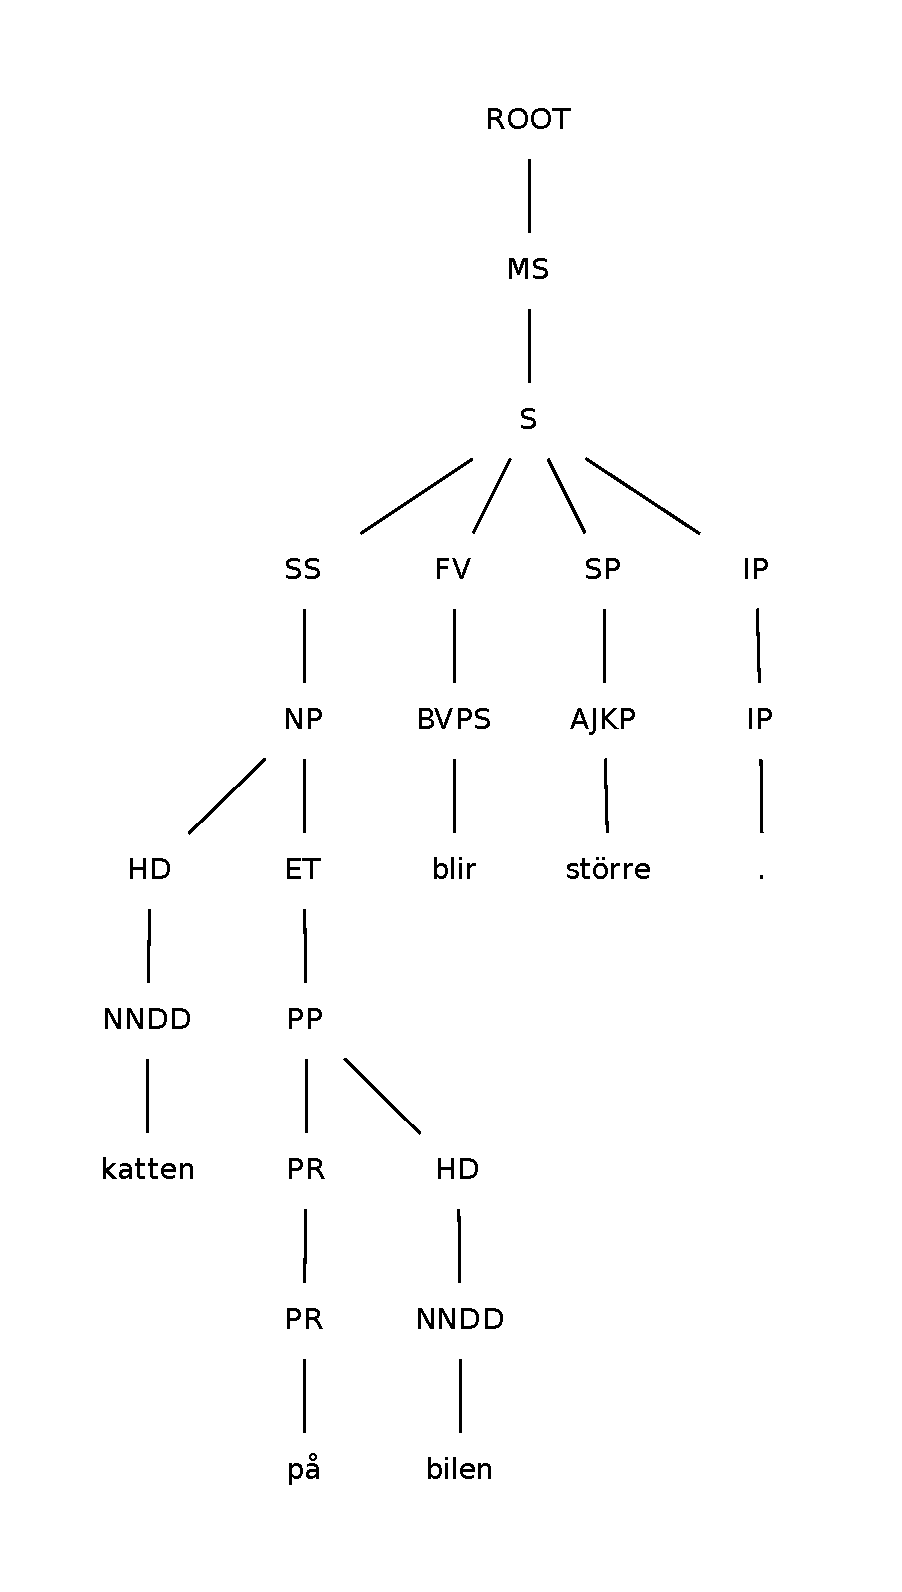
\includegraphics[width=60mm]{Talbankentree.pdf}}
\hspace{-10mm}
\subfloat[GF abstract tree]{\label{pic:gftree}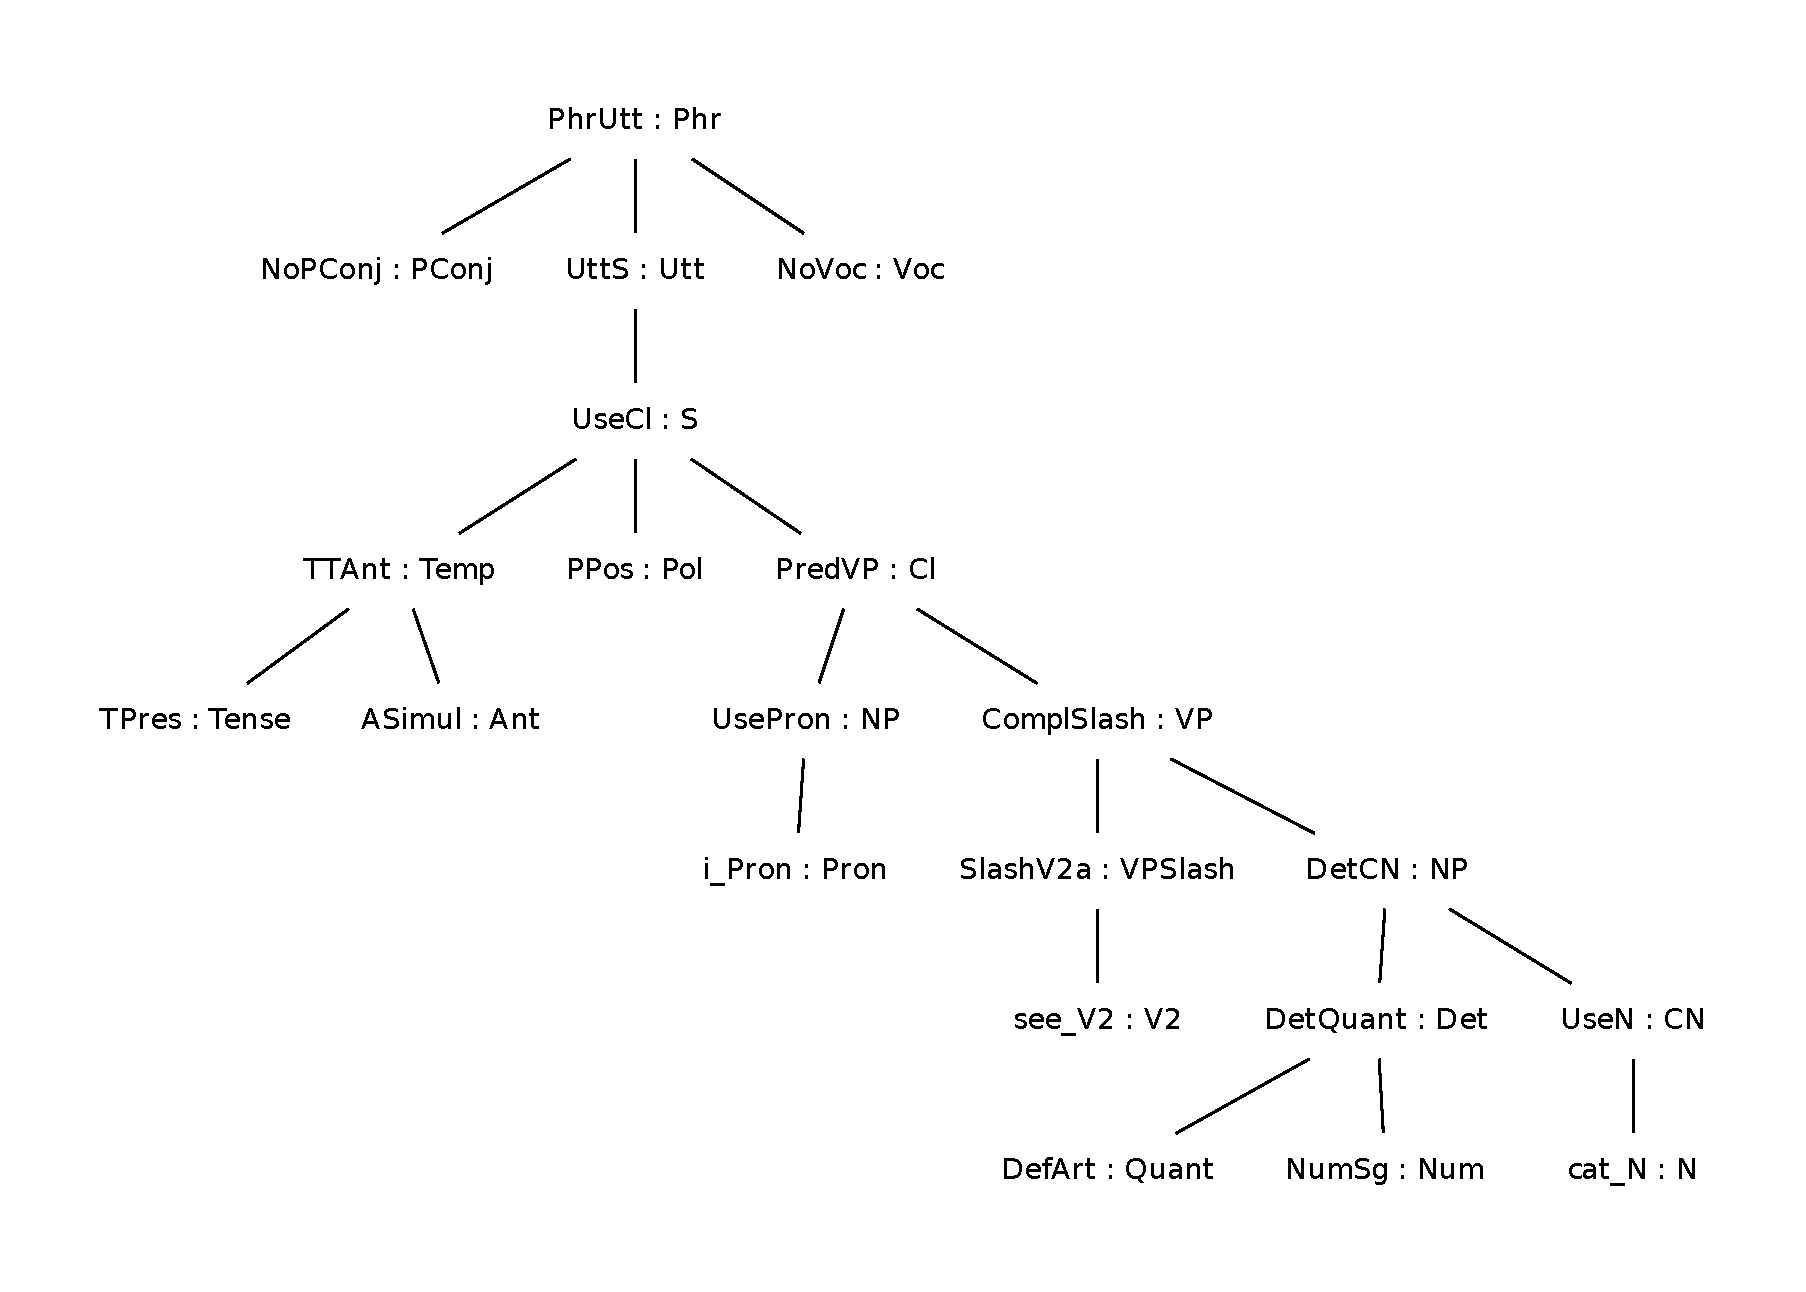
\includegraphics[width=100mm]{gfTree.pdf}}
\subfloat[The corresponding GF parse tree]{\label{pic:gfptree}\includegraphics[width=50mm]{gfPTree.pdf}}
\caption{Trees for the sentence ``Katten på bilen blir större".}
\label{fig:translationtrees}
\end{figure}

The mapping %connects GF with another annotations and 
gives us means to evaluate our parser. By both parsing a Talbanken sentence and
transforming its annotated tree, we can easily inspect if the results are
equal.
Additionally, the mapping shows which grammatical constructions that are still missing
from the GF grammar and shows how the GF analysis differs from the one made
in Talbanken.
If there are words missing from our dictionary, the rich
POS-tags may help us to automatically find the correct declination and add it to the
lexicon. Further, our parser will need probabilities (see section
\ref{sec:future}) of how often a function is used. The GF treebank we
achieve from the translation is a good source for this information.\\
%missing words. Lexical aquisation, probabilities, see section .
%The mapping gives information about which form a word is
%currently used in and this may be used by the lexical extraction
%tools. % Those can be enhanced if they are given more data. 
%The translated trees enable us to extract those probabilities. %The mapping gives us a source for this.
%Furthermore, the translation makes it easy to identify grammatical constructions
%missing from the GF grammar Another important use of the mapping is evaluation of the parser, which can be
%accomplished by comparing the parse trees and the trees from the transformer.

The mapping is based on 
a translation of the English Penn Treebank \cite{gfpenn}.
By modifying this program, we now have a translation that works for
the Tiger XML-format of
Talbanken. Adaption was required for the differences in annotation as well as 
for the syntactic differences between Swedish and English.

%The mapping works for Talbanken05 in Tiger XML-format.
\section{The Talbanken annotation}
Talbanken05 uses three kinds of tags: categories, edge labels and pos-tags. 
%TODO part of speech??
While the pos-tags are reserved for words, the categories give part-of-speech information,
such as \verb|S|, \verb|NP| and \verb|VP|.
The edge labels give the grammatical functions: \verb|SS| for subject, 
\verb|OO| for object etc. Nearly 400 different tags are used, of which more than
300 different are pos-tags. The high number is due to the level of detail,  there are for
example almost 50 tags for nouns, excluding proper names. The tags
show definiteness, case and whether the word is a compound. Some words also have
their own tags.\\

\begin{tabular}{lll}
\textbf{Tag} & \textbf{Example} & \textbf{Explanation} \\
\hline
\textbf{SV} & ska & The verb \emph{shall}\\
\textbf{WVIV} & vilja & The verb \emph{want} in infinitive\\
\textbf{KVSP} & kommit att & The future auxiliary verb \emph{kommer} in supine\\
\textbf{GVPT  PA} & gjordes & The verb \emph{do, make}, present, passive \\
\textbf{NNDDHSGG} & familjemedlemmarnas & Noun, definite, compound (person), genitive \\
\textbf{PU} & * \; 1) \; a) & List item\\
\end{tabular}\\

%Pos continues
%to either new tree or a word. Example S -> PP -> (Hd -> Id , Hd -> Id). Show
%corresponding GF tree.

\section{The translation process}
The implementation consists of a set of rules that translates
one node of a Talbanken tree to a GF function, possibly by describing what the
nodes subtree should look like. 
\begin{verbatim}
translate S  = do
             np <- find NP
             vp <- find VP
             return (PredVP np vp)
\end{verbatim}
This rule tells that we may map the category \verb-S- to the function 
\verb-PredVP-, given that we find a noun phrase and a verb phrase in
the subtree of \verb-S-.

At every leaf a word is given. %When a leaf is reached,and ato see if
It is looked-up in the GF lexicon and the result compared to the information of
the pos-tag.
If the word is not found in the lexicon
a \textit{meta} variable will be put in its place, denoted `\verb-?-'.
The meta variable is also used when we have found two translatable trees
but no rule that allows them to be combined.

Lets look at the example in figure
\ref{pic:tbtree}. The verb \emph{``bli"} is
followed by a predicative 
adjective modifying the subject, \verb|SP|. GF admits \emph{``bli"} to have
type \verb|VA|, a verb with an adjective as complement, and the translator can
apply the GF function \verb|ComplVA| to combine the verb with its object. \\

The translation covers complex noun phrases which may consist of pronouns,
reflexive objects or common nouns and contain predeterminers, 
determiners, quantifiers and adjectival modifiers. Special rules were needed
for each verb category in order to find the right number of arguments.
The mapping also covers different word order, such as questions and topicalisation.

%The translation works section-wise, ie. if it finds a tree of category 
%it will start to look for a subject \verb|SS| and a finite verb \verb|FV|. If it
%can find those, they can be combine with the GF function \verb|PredVP|.
%It is not always the case that we first find the subject, then the verb and 
%finally the objects. Often the order is Verb-Subject-Object or Object-Subject-Verb. \\
%During the mapping process, the translator also needs to find out whether the sentence is
%negated and what tense is used. If it finds two trees of type, say, \verb|VP| but does not
%have any rules for combining them, the \textit{meta function} \verb-?- will be used. 
%Figure xx shows an example of this.\\

%How we try to build up a 'abstract syntax tree', a S with a NP VP for example. 
%Continue with dividing VP into Verb Objs. More possible word orders (or at
%least more commonly used). 'katten åt sin mat fort' 'åt katten sin mat fort' 'sin mat åt katten fort'
% If can't find, add a '?', a meta.
%This is also what happens when the translator finds a combination it doesn't know about.
%Example of tree with meta.

%Description of most important tags from Talbanken, their translation? appendix?
\subsection{Differences in the notation}
Some structural differences between GF and Talbanken became obvious during the
translation.
%Since the translation is done word by word, ambiguities may confuse the translator.\\
%shown during the translation.
%cause some translation problems.
In Talbanken the valency information is given implicitly by the complements
of a word. If a verb is followed by an object, \verb-OO-, which contains an
\verb-S-, we can conclude that this is a sentence-complement verb.
In GF, the valency information is given for each entry in the lexicon.
A sentence-complement verb has the type \verb-VS- and from this we know 
that the function \verb-ComplVS- should be used to combine the verb and with a 
sentence.
\begin{wrapfigure}{l}{0.52\textwidth}
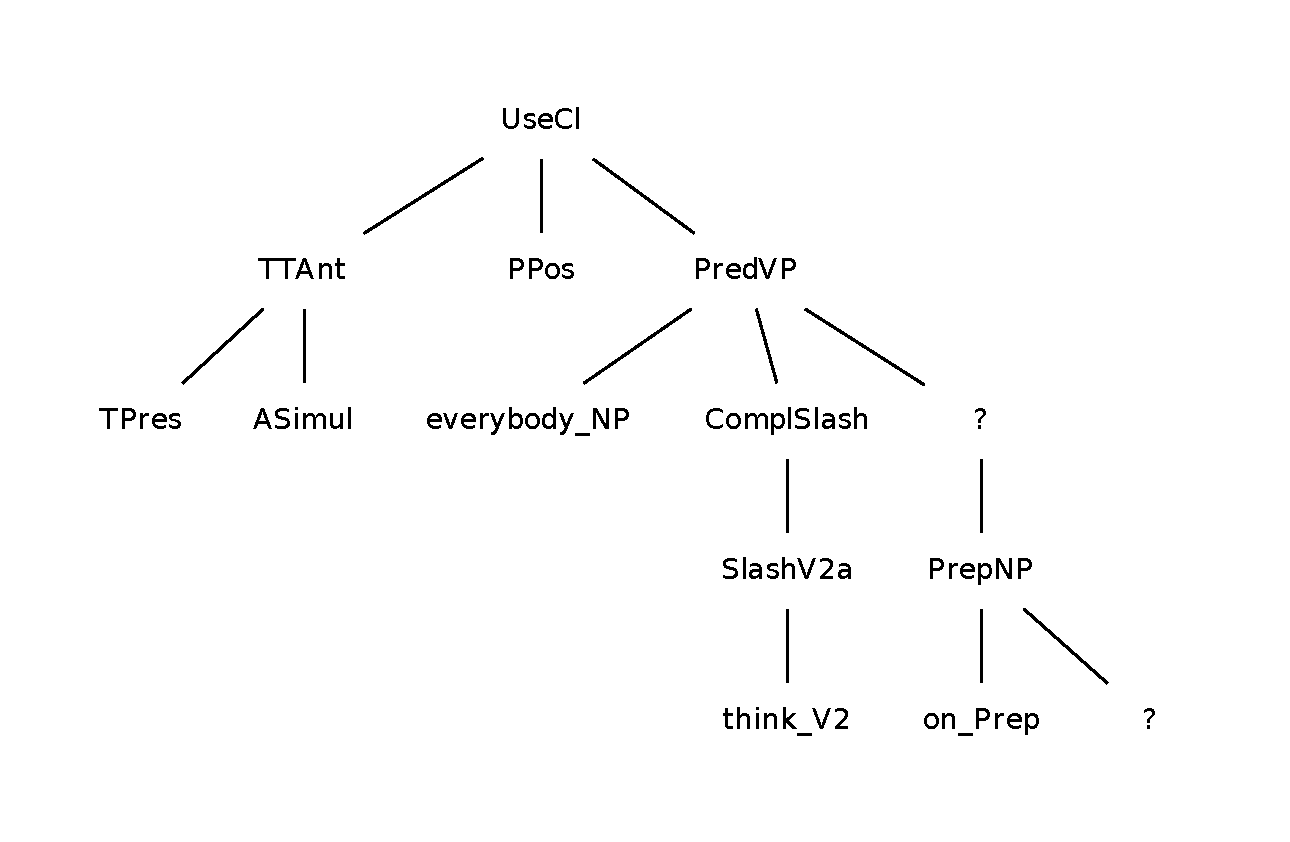
\includegraphics[width=80mm]{metatree.pdf}
\caption{Abstract tree with meta}
\label{pic:gMetatree}
\end{wrapfigure}

A similar issue arises from the use of verb particles. A verb with a
particle is treated as two independent units in Talbanken but in GF they are
considered to be one constituent. % which means that 
The particle has therefore no effect on the abstract tree, its presence is
announced by the verb itself.

%In Talbanken, verbs and particles are treated as separate units,
%and the particle is marked with the tag \verb-PL- and attached to. 
%Talbanken has no valence information while this is crucial for GF.
%The grammar requires a adjective-complement verb,
%\verb|VA|, to be used with one adjectival phrase. For \emph{``bli"} in example
%\ref{pic:tbtree}, we know that we need to find an adjective phrase.
%%know what kind of verb we are looking for
%%when consulting the GF lexicon.
%If the GF lexicon assings different types to verb, the correct type 
%should be showed by the complements.
%This way %\enumsentence{Han gillar det\\He likes it} 
When constructing the abstract trees, we must of course follow and use the
GF analysis. However,
the mapping cannot depend on the valencies given in GF only, 
\newpage



\noindent since the distinction between different types of verbs is not always clear in Swedish;
most transitive verbs can also be used as intransitive. Both sentences in
example \ref{ex:mappTransitive} are grammatically correct but only (\ref{ex:mappTransitive}b)
is accepted by the GF grammar, and
the grammar rules are simply too strict for accepting many Talbanken sentences.
\enumsentence{\begin{tabular}[t]{@{}*{14}{l@{\ }}}
a. &Han& sitter& och &läser.&& & b. &Han& sitter& och& läser& en& bok.\\
&\emph{he}& \emph{sits}& \emph{and} &\emph{reads} &&&
&\emph{he}& \emph{sits}& \emph{and}& \emph{reads}& \emph{a}& \emph{book}\\
\end{tabular}}
\label{ex:mappTransitive}
See section \ref{sec:futureValency} for a longer discussion about this.\\
%the Talbankenwill allow words to be used in other ways than their
%GF valencies prescribes.

Another annotational difference that turned out to be problematic for the
translation can be illustrated by sentence (\ref{ex:mappMan}), containing
the generic pronoun \emph{``man"}.
\enumsentence{
\shortex{3}{Man & uppskattar & dem}
{\emph{one} & \emph{appreciates} & \emph{them}}
{``They are appreciated"}}\label{ex:mappMan} %  (s216).

In Talbanken, \emph{``man"} is simply a personal pronoun, 
in GF it is represented by using the function \verb|GenericCl|, see figure
\ref{fig:mappMan}. \verb|GenericCl| turns a \verb-VP- into a clause and has no
subject visible in the abstract tree. 
\begin{figure}[h]
\centering
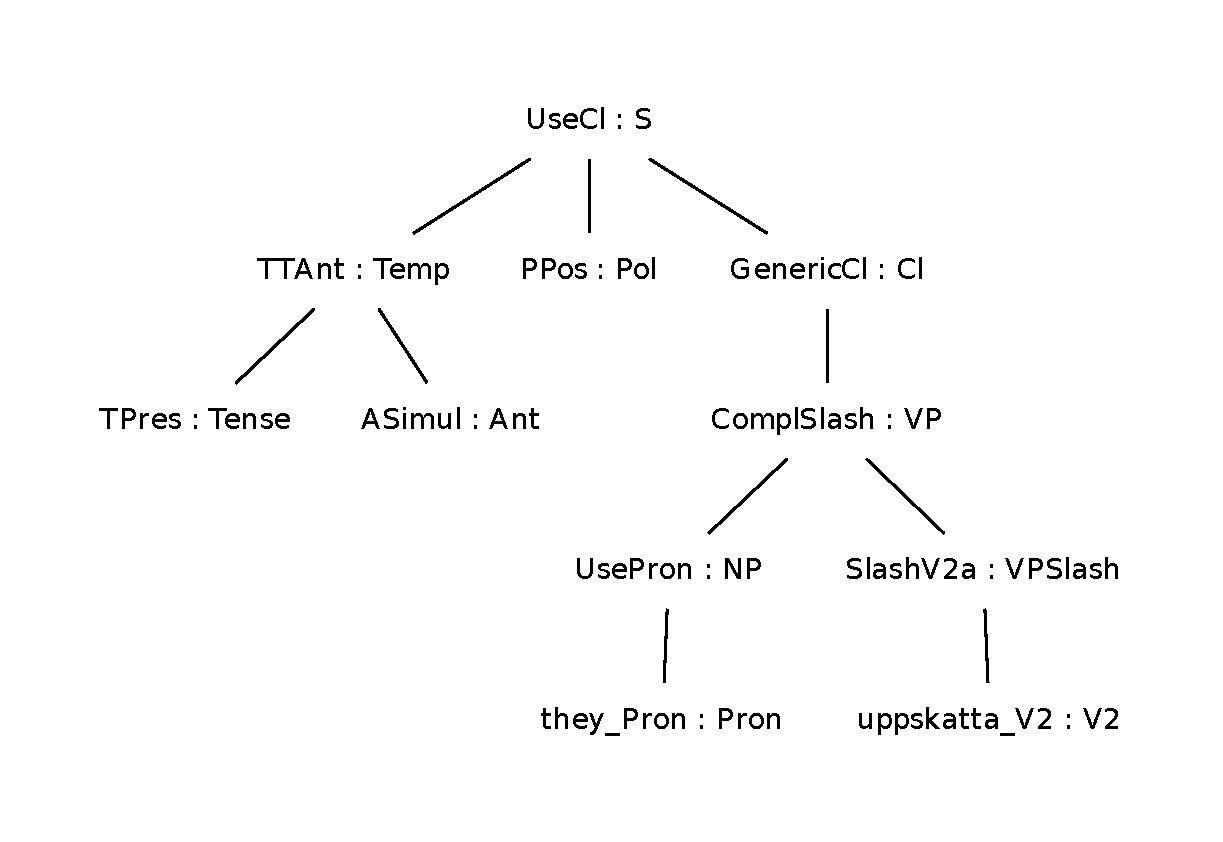
\includegraphics[width=80mm]{man.pdf}
\caption{Abstract tree for ``Man uppskattar dem".}
\label{fig:mappMan}
\end{figure}
When translating a sentence like this, it is thus not possible to simply glue the
subject to the verb with \verb|PredVP|. For each similar GF construction, an extra rule
would be needed to get full coverage. \\ %and the normal top-down? approach fails.\\
%Therefore, the translator must change the type of the 
%sentence when inside the SS.

%The lexicon may contain a verb both with and without a particle,
%for example \emph{tänka} (``think") and \emph{tänka till} (``consider").
%\begin{verbatim}
%taenka_V  : V ;
%taenka_till_V : V ;
%\end{verbatim}
%When the translator looks up a the form \emph{tänka}, both of the two verbs
%will be among the results. %It is not known until later which one 
%%The first option will be selected, and if the
%%particle isn't directly attached to the verb
%%There is, at this point, no easy way of knowing which one of them wants a particle and the
%the transformation might confuse the two words. This is also the case when translating
%all sorts of idioms that GF considers to be just one bit.\\
%
%Difficulties in looking up 'idioms' like this
%in the gf lexicon. Therefore the translator might get confused.
%Sentences are also differntly deep. Example of a conjuncted sentence.

\section{Results and evaluation}
%>> more! replace words, how much better results (both grammar and mapping) 
%>> more results
%>> motivation, why so bad??\\
The development was mostly example-driven, and at least one rule for the translation of
every Talbanken-tag has been implemented.
Shorter sentences have been prioritized in order to get a coverage of the most
fundamental constructions. 
Regression testing was used to ensure that a new rule would not violate the old ones
or allow trees to be translated erroneously.


The flat version of Talbanken05 was used for developing the mapping, but
the program works for both the flat and the deep Tiger-XML versions.
The deeper contains six more tags, although they are not always useful for our       
purpose. Figure \ref{fig:mappDeepFlat} shows the difference for a conjunction.
% show piece of s5 here!
\begin{figure}[h]
\begin{parsetree}
    ( .CNP. 
        (.CJ.  (.NP. ~ `oskifta dödsbon'))
        ( .++. (.++OC. `och'))
        (.CJ.  (.VN. `familjestiftelser'))
    )
\end{parsetree}
\begin{parsetree}
    ( .CNP. 
        (.CJ.  (.NP. ~ `oskifta dödsbon'))
        ( .CC.
            (.CNP. 
                (.++.  (.++OC. `och' ))
                (.C+.  (.VN. `familjestiftelser'))
         ))
    )
\end{parsetree}
\caption{An example of the difference in the two analyses}
\label{fig:mappDeepFlat}
\end{figure}

Some more information about VP are given by the tag \verb|VG| (\emph{verb group}),
which groups an infinitival verb and its object together into a \verb|VP|.
This information can however be extracted from the flat version, and the results
get slightly better when using the flat version. \\


When evaluating the mapping, the results strongly depend on which restrictions we
put on the input. 
One of the reasons why a node cannot be translated, is the 
use of the tags show in figure \ref{fig:mapBadtag}.
The \textbf{PU} tag is used for graphic listings, and not for fluent text.
In our grammar there is naturally no corresponding function; 
%We are not interested in sentences made up by list, since 
the listings are meant for making the text look nice in
folders etc and outside the scope for the grammar itself. The tags \textbf{XX} and \textbf{NP} are often used since
Talbanken -- unlike GF -- makes a difference between subjects
and objects. %(which is not needed in GF (see section \ref{sec:swegf}))
The analysis of elliptical expression in (\ref{sent:krav})
\enumsentence{För stora krav.\\
``Too high demands."}\label{sent:krav}
contains the tags \textbf{XX} and \textbf{NP}, since it is not obvious
whether the noun phrase is used as subject or an object.
The tags shown in figure \ref{fig:mapBadtag} occur quite frequently in the treebank and are always translated
to metas, which lowers our result. \\
%How we cannot cover all cases. 
\begin{figure}[h]
\begin{tabular}{ll}
\textbf{NAC} & Not a constituent\\
\textbf{XP} & Other (non-coordinated) phrase\\
\textbf{DB} & Doubled function\\
\textbf{PU} & List item\\
\textbf{XX} & Unclassifiable part-of-speech\\
\end{tabular}
\caption{}\label{fig:mapBadtag}
\end{figure}


Our focus has been on shorter sentences, with no idioms or conjunction.
If we assure that the lexicon contains the correct word class for all lemmas
involved, we
can restore more than 85 \% of the nodes in the original tree.
If we lift all the restrictions excluding the \verb|PU|, we get
%When tested the 100 first sentences from Talbanken, we get
65 \% coverage. 
If we test randomly collected sentences that do not contain any of the tags listed
in figure \ref{fig:mapBadtag}, 72 \% can be restored (see figure \ref{tab:mappres})

%TODO
%All NPs: 72%
\begin{figure}[h]
\begin{tabular}{|ll|}
\hline
No list items & 65 \%\\
No special punctuation or bad tags& 72 \%\\
Short sentences with known words & 85 \%\\
\hline
\end{tabular}
\caption{}
\label{tab:mappres}
\end{figure}

A mapping between GF and the Wall Street Journal of Penn Treebank has earlier been conducted \cite{gfMech}.
The percentage of restored nodes from Peen Treebank is higher than our results.
%TODO review
The reason for this may be the fact that English is syntactically less complicated
than Swedish.
Furthermore, the text in Talbanken are from various brochures, newspapers and text books,
where idiomatic expressions are more likely and the language presumably less strict than
in Wall Street Journal.
Also, the Penn Treebank contains a lower number of tags, 82 compared
to more than 300 in Talbanken. Even if the tags describing the same word
%TODO review
class as another tag are excluded, Talbanken still leaves us with more than 130 tags.
With more tags, we get more information, but as the number 
%Thus the number of
increase, so does the amount of work of finding the correct translation 
for each combination of tags and writing rules that cover all constructions. 
%iand so is the number of
%rules that would be needed to cover all constructions.

We believe that the results could be enhanced by simply adding more rules 
and in this way get a wider coverage. There are many special cases that require
special rules. Since we are not aware of any formal specification of how the tags may be
combined in Talbanken, the only way of finding all possibilities are to manually look
for different patterns. Another option would be to make the mapping more
robust, but the robustness must not interfere with the correctness.

% compared to penn treebank: 82 tags. talbanken: at least 130
% 99.1 % of Penn sentences have 6 or fewer clauses

%If we don't take the verb valency into account, allow all verbs to have Gf category V,
%we get a slightly better result,
%from 62.5 \% to 65.4 \%.  (see EvalText). The complemnt of the verbs should tell which category
%they are anyway.
%Evaluation. -> Works for both flat and deep, but with sligthly better results for the flat one.

% hard examples like
% ger sig till henne -> ReflSlash ge henne in gf
% questions with objects that should be moved
% vilken katt såg du
%This part explains
%the tags in Talbanken and gives examples of how they are translated,
%examples of what can be parsed and what cannot.
%about how to make the code work for swedish, differences
%regression testing


\chapter{Discussion}
\label{sec:results}
\section{Evaluation}
%TODO
%>>evolution diagram?
%also removed unnecessary ambigutiies.
%>> how to handle ambigs: know them and controll them. using statistics or ontolgies.
%>> that is: disambiguitation by context or by meaning.
The project has resulted in
\begin{itemize}
\item a large-scale GF lexicon and a program to redo the importation when needed
\item a comparison between GF and another another annotation
\item a deeper testing of the Swedish resource grammar and an estimation
of how well GF can be used to describe larger parts of a language
\item a study of how dependent types can be used in the resource grammars
\end{itemize}

The grammar has been extended and enhanced, and its current status is
a specialized extension of the resource grammar.
Besides parsing, the grammar may well be used for language generation,
which is fast even with an extensive lexicon.
%TODO make nice!
Although it cannot not been verified, we believe that the majority of the
sentences generated are grammatically correct in a syntactical point of view.
Without any semantical knowledge, nonsense phrases cannot be avoided in
random generation. However, given that the abstract tree has a meaningful
interpretation,
%TODO move to Misc?
the linearization should be correct. There are some cases when the correctness
of the output has been put aside in order to increase the expressivity, such
as \verb-ComplBareVV-, which use a verb-complement verb without the inifite mark, 
as in sentence (\ref{sent:complVV1}b).
\eenumsentence{\item\shortex{5}
{Jag& börjar&\textbf{att}& bli& hungrig}
{\emph{I}& \emph{begin}& \textbf{\emph{to}}&\emph{become}& \emph{hungry}}
{I'm getting hungry}
\item
\shortex{4}
{Jag& börjar& bli& hungrig}
{\emph{I}& \emph{begin}& \emph{become}& \emph{hungry}}
{I'm getting hungry}}\label{sent:complVV1}
Since there is no information about which verbs that allows the inifinite mark
to be left out, it will also allow the more questionable sentence (\ref{sent:complVV2}b).
\eenumsentence{
\item \shortex{5}
{Jag & vill & \textbf{att}& du & går} 
{I & want & \textbf{to} &you & leave}
{I want you to leave}
\item \shortexnt{4}
{Jag & vill & du & går} 
{I & want &you & leave}}\label{sent:complVV2}
%ComplBareVV, SupCl
For random generation, the sentences generated may be next to impossible
to interpret without looking at the abstract tree, since they may contain
too many attributes, relative clauses etc. 
%\enumsentence{Kommer övriga datorer idag som ska vara inte att ha målats?}
%\label{sent:what}
%Sentence (\ref{sent:what})
%PredVP (DetCN Subject (DetSub oovriga_Det) (RelCN (AdvCN (UseN computer_N) (AdvSub today_Adv)) (UseRCl (TTAnt TFut ASimul) PPos (RelVP IdRP UseCopula)))) (PassVP (SlashV2A paint_V2A (ComparA Object red_A (UsePN Object johan_PN))))
%The use of the NONEXIST pattern, as described in \ref{sec:Formal}. When using
%the grammar for generation, an extra 

When it comes to parsing, we do not get far without robustness.
The grammar in itself is by no means robust, and just one 
unexpected punctuation mark, unknown word
or ellipsis will cause the parsing of the whole sentence to fail. 


Parsing bigger parts of Talbanken would hence give very low results at this stage, 
%, for the reasons stated.
and a comparison of the results would not be of much value as
there would not be enough material %underlag is yet too small 
to do be able to do any interesting analysis.
An estimation of the improvement can be given by looking at the results from
running the test suite used for the grammar development.
The sentences given in the test suite are short, four to 10 words, and the
words are in most cases included in
the lexicon, but there are also constructions that have not been implemented 
during this project.
The first grammar could parse almost half of the sentences, the result for the final
grammar was 66 \%. 
% try NPs?
It is thus not yet interesting to talk about coverage, but about the quality and
the ability to scale up, which has so far proved to be good.
I further believe that the presence of a expert in Swedish, professor Elisabet
Engdahl\footnote{http://svenska.gu.se/om-oss/personal/elisabet-engdahl},
has
increased the standard substantially.\\


By the renewed import of Saldo, we have doubled the size of the lexicon and thereby
added many of the commonly used words that were missing from the older
version. This is of course a big improvement.
However, the lexical part still requires much work before it can be made use of.
We need valency information to make a good analysis. The lexicon is also too
big to use with the current techniques. Its size causes the
incremental parsing algorithm to use more heap memory than normal computers
allow. To solve this, we need to use the lexicon data more cleverly.

%Results from mapping, can probably be improved, bit by bit, depends much on words.
%Valencys would therefore help.  
%Saldo, made a big difference to renew the lexicon. Tested what was missing now from talbanken,
%results. Mostly compound nouns, which we can't expect in the dictionary.
%Is too slow, can't be used for parsing right away
%
%Grammar - hard to evaluate automatically, but Elibet is an expert who has been involved
%in the process to verify the solutions. Testing trees against talbanken.
%The big lexicon makes it very slow, eats all memory
%
%Discussion of the results and methods, why are the results good, why are they not better.
%What other methods could have been used? What did we/I expect and what happend?

\section{Future Work}
\label{sec:future}
At the end of the current project,
%Having finished this part of the project,
we are left with 
%Although this one part of the project is finished, there are 
many interesting future directions.
The future work described in this section is divided into two categories:
the ones aiming at making the parser robust and the ones that can be
seen as extensions of the work done so far.
 
\subsection{Enhancements and complements}
\subsubsection{Grammar}
The grammar should cover the most prominent Swedish features.
%All imaginable grammatical constructs cannot be cover by our grammar.
Some work must be left for the robustness, but there are specific constructs
that are desirable and interesting to implement. A few examples are listed here:\\

\begin{itemize}
\item
\textit{Pronominal object shift} is common in Swedish and obligatory in Danish and Norwegian.
\enumsentence{\begin{tabular}[t]{@{}*{11}{l@{\ }}}
a. & Jag & ser&  honom& \textbf{inte}&~~ & b.&Jag &ser &\textbf{inte} &honom\\
   & \emph{I} & \emph{see}&\emph{him}&\emph{not}&&& \emph{I} &\emph{see}&\emph{not}&\emph{him}\\
\end{tabular}}
Personal pronouns are allowed to precede negation and some other sentence adverbials --\textit{satsadverbial} --
in main clauses without auxiliary verbs.

\enumsentence{\begin{tabular}[t]{@{}*{12}{l@{\ }}}
a. & *Vi & har&  honom&  inte&sett&~~ & b.& * Jag &ser &huset &inte\\
   & \emph{~we} & \emph{have}&  \emph{him}&  \emph{not} &  \emph{seen} && b.& \emph{~I}&\emph{see} &\emph{the house} &\emph{not}\\
\end{tabular}}

Although object shifts are frequently used, they are hardly found in
Talbanken's part P, which has been the inspiration for this project.
Therefore, this implementation has so far not been prioritized.\\


%Sentences like
%'hon är inte dum, hon.' 'hon är inte dum, flickan' 'min syster, hon är inte dum, hon'
%'min syster är inte dum, hon'
%We have a clause of which we need to know the natural gender and number of the subject, since it
%must agree with the added pronoun. sag s 439. fullständigt outforskade!

%or just implement this and remove it here?
%The question is how many types we should give dependent types. CN could also need it,
%in order to say
%'han mäter avståndet från sitt hus till sitt jobb' but now `avståndet från sitt hus är stort'.
%The analysis of this sentence is that
%avståndet is a noun of type \verb-N3-, which chooses the prepositions ``från" and ``till"
%and needs to noun phrases to form a \verb-CN- -- ``avståndet från sitt hus till".
%Now also \verb-CN- needs to carry about whether it is possible to use it as a subject.

\item
\textit{Bare indefinites} are at this point always parsed as mass nouns.
\enumsentence{\shortexnt{3}
{Jag & dricker& vatten}
{\emph{I}&\emph{drink}&\emph{water}}
}\label{sent:water}
The parse tree of sentence (\ref{sent:water}) looks as follows:
\begin{verbatim}
PredVP (UsePron i_Pron) (ComplSlash (SlashV2a drink_V2) 
                                      (MassNP (UseN water_N))) 
\end{verbatim}

This however is not the correct analysis for `hund' (\emph{`dog'}) in sentence (\ref{sent:hund}).
\enumsentence{\shortex{4}
{Vi & ska& köpa & hund}
{\emph{we} &\emph{will}& \emph{buy} & \emph{dog} }
{We are going to buy a dog}}\label{sent:hund}

\item
The implementation of reflexive pronouns can be improved.  %both code-wise
It should for example be possible to differentiate between 
object and subject control verbs.

\eenumsentence{
\item[a]\shortex{7}
{Han & ber & henne & att & städa & sitt & rum}
{\emph{he} & \emph{begs} & \emph{her} & \emph{to} & \emph{clean} & {\sc self's} & \emph{room}}
{`He asks her to clean her room'}
\item[b]\shortex{7}
{Han& lovar& henne& att& städa &sitt & rum}
{\emph{he}& \emph{promises}& \emph{her}& \emph{to}&  \emph{clean} &\sc self's&\emph{room}}
{`He promises her to clean his room'}}

%
%\verb| X : NP x + CN + NP --better|\\
%\verb| X : CN x + CN + CN|
%check apposCN.
%\textbf{måttsattribut}
%\enumsentence{
%{Antalet bilar, ett antal bilar, ett stort antal}}
%Genitive; Not like 'sonen till mig' -> antalet bilars??\\

\end{itemize}
\subsubsection{Lexicon}
Our lexicon still lacks some parts that can be imported from Saldo.
The multiple-word verbs (\verb-vbm-) and multiple-word nouns (\verb-nm-) should
be imported to an idiom lexicon, which can be used as an extension to the main
lexicon.
For the words that we tried but failed to import, another tool for lexicon
acquisition could be used. The tool developed in the previous part of
this project\footnote{??} would be suitable.
All in all, it should be ensured that we use as much information as
possible from our resources.
%The list of not-imported can be used for adding other kinds of lexicons - idioms, have pos-tags.
%Also to analyse what's wrong, or use the words with a word guesser. The code
%has been adapted for this.
%For exapmle pronouns - dets, have combined information from Talbanken to add them in the correct
%category. How this works, look at tags. Small amount, can be done manually.


\subsection{Making the parser robust}
To achieve our goal of parsing unrestricted text, we need to use statistical methods.
The parser needs to be able to handle
ellipses and long sentences, names and numbers,
compound words and unknown constructions.

\subsubsection{Parallel parsing/Chunk parsing}
Instead of parsing a whole sentence in one go, we would like to
parse parts of it in parallel and then try to combine the pieces.
This method should be faster then normal parsing and would
at the same time give robustness;
components that cannot be combined by any grammar rule are combined by a 
meta function. When an unknown construction is encountered, the parser
will not fail but give a partial parse tree with the analysis for the rest of
the sentence \cite{gfMech}.
The output given to the user will be more valuable, since partial parse
trees are more interesting the no parse trees.
%We might end up with partial parse trees, but we would
%be able to parse at least parts of every sentence and give a more
%interesting result to the user.

\subsubsection{Lexicon}
\label{sec:futureValency}
No matter how much we increase the size of our lexicon, we will
never cover all compounds. We therefore need to be able to do
compounding analysis. Saldo has tools for this, which might be usable
in this project as well \cite{fm}.
As noted, we additionally need to come up with better methods for using the lexicon when
parsing, since its time and memory consumption is very high.
One possibility is of course to do 
deeper refinements of the parsing source code, an extensive work which is far
outside the scope for this project. Other solutions are to either
adapt the lexicon automatically for its domain and hence making it smaller and
faster, or to adapt the input sentences to a smaller lexicon by preprocessing.

Further, the lexicon needs valencies since this information lays the
foundation for the GF analysis. 
During the mapping, described in section \ref{sec:Mapping}, we analysed how Talbanken
annotates valency information. It should be possible to %extract data from %and by using the rules made for the mapping
extract data from Talbanken,
showing how words are normally used. There should also be algorithms for
automatically adding the information to the lexicon. \\
Many Swedish verbs can be used with different number of arguments.
Having one lexical entry for every possible usage of a verb
%all this information to the lexicon 
does not seem to be a good idea considering
the ambiguities it will lead to and the already high time usage.
The task should instead be left to the robust layer of the parser, possibly
implemented by using external resources.
% TODO like what?



%how to get valency information 'sitter och läser',
%is this doable for swedish?
%description of extracting this from talbanken/korp
%or handling it by the robust parser or the grammar itself (leaveout obj?).
%make the parser faster by using smaller lexicon.
%Lexicon tool on the fly.

\subsubsection{Probabilities}
\label{sec:futureProbabilities}
The grammar will always contain ambiguities and before returning the result
to the user, some analysis should be done to find the most probable tree.
When the size of the lexicon
increases, so will the ambiguities as the number of word forms overlapping each other
gets higher. Our new grammar also have many more rules which contribute
to increasing the number of interpretations of each sentence.

GF already allows probabilities, and by using a large
GF treebank, we can get more reliable statistics for our functions. 
By implementing dependency probabilities, our results would be even better.

%TODO
%The many word forms in the gF tables, as seen in section \ref{saldo}.
%This is a possible source for overgeneration.
\subsubsection{Named entity recognition}
The parser should be able to identify names of persons, companies, countries etc.
This can be done by the Haskell program executing the parsing \cite{patent}.

% discuss ambiguites, will always have some and the big lexicon will increase them.
% exapmle 'vad händer under äktenskapet?'
%Getting and using probabilities, to disambiguate.
% ontologies?


%Use multiligual treebank



\section{Conclusion}
%>> why is this significant, other grammars can use this Swedish grammar.
%>> robustness in in future work leads to coverage.
%>> reusablilty, freely available.
%TODO
%>> well known (comp. ling) trade-off between depth and coverage. for now depth,
%>> have experiments of how to extract info from talbanken.\\


We have developed the main components
for a deep Swedish parser; an extended grammar and lexicon and material for
evaluation and disambiguation. %To abstract:  by combining resources.
We started from a well-defined system for describing grammars as we built
the grammar from the GF resource grammar.

%When parser is derived from the grammar and will therefore validate that
%a given sentence is grammatically correct according to the rules defined.

Our final goal is to be able to parse unrestricted text, but considering that
no syntactic theory is yet capable
of wholy covering a natural language, we are satisfied with %theconsider our grammar 
%when used without a robust layer 
the grammar implementation of an important fragment of Swedish.
We have therefore focused on constructions that are frequent in Talbanken, 
and following methods for making the parser robust as described in section \ref{sec:future}
we still believe that it is possible to achieve the goal. 
\\

%TODO more here
Being a natural language processing-project, it will probably never be
entirely complete. Even so, we believe  
%Even though the grammar will not be totally covering, we belive
that the work done is both interesting and useful.
All parts of the project are open-source and may thus be used in other applications.
The grammar may be beneficial also when working with controlled languages,
as it increases the coverage of the Swedish resource grammar.

The constructions
that we have focused on have all been possible to implement, with varying  amounts
of work. Many of them could be done by utilizing and extending the resource library
but in some cases we needed to part from the multilingual abstract and use other
grammatical theories in order to arrive at a good analysis.




%There is obviously a lot do still, will never get finish with NPL.
%Grammar may need even bigger changes, to allow enough but not too much.
%Different from writing a grammar for generation.
%Results from mapping shows that the translation is doable, but becomes harder
%since talbanken don't have formal rules.
%The saldo shows how easy to make use of utomstående resources, promising if
%we want to extract other information. 
%Hard, but not finished! 

%TODO Espana -> ~
\bibliographystyle{apalikeurl}
\bibliography{masterbib}
\end{document}
